\section{Evaluation results}
\label{sec:ch4-report}

The report generated by fuzzbench collecting the coverage information is placed in \texttt{report-data} directory, beside the experiment files located in \texttt{xp-data}. The reports are generated in figures and an HTML file for illustrating the results. We first analyze the code coverages, and then we examine the execution times.

\subsection{Code coverage}

\subsubsection{Code coverage growth}

Figure \ref{fig:cov-growth} shows the code coverage growth of the fuzzers, while fuzzing each benchmark. There are three trials for each fuzzer, and the illustration shows the highest code coverage, the minimum code coverage, and the median of the trials' results. AFL++ shows a significant better performance than other benchmarks. In fact, AFL++ is has the highest performance in coverage among all other benchmarks which are provided in fuzzbench project. Waffle, as expected, is seemingly performing same as AFL. This is followed by the fact that Waffle performs the same code coverage approach, but there are new different features for producing queue entries. In \ref{fig:sub:freetype-cov-growth}, the trials of Waffle show more variance in performance. Hence, AFL's trials grow close to each other. In the paper based on fuzzbench results \cite{metzman2021fuzzbench}, the \texttt{deterministic stages} of AFL's fuzzing is behind such performance. It is also noticeable that Waffle discovers significantly more regions in at least one of the trials. Testing libjpeg-turbo-07-2017 (Figure \ref{fig:sub:libjpeg-cov-growth}) and libpng-1.2.56 (Figure \ref{fig:sub:libpng-cov-growth}) show a close performance for AFL, AFLFast, and Waffle \ref{fig:sub:libjpeg-cov-growth}. Another interesting result collected from fuzzing libxml2-v2.9.2 suggests a difficulty for Waffle in exploring the code coverage, but eventually Waffle gets the pace closer to other fuzzers. In addition, AFL is the winner of the 4th experiment.

\begin{figure}
    \centering
    \begin{subfigure}[t]{\textwidth}
        \centering
        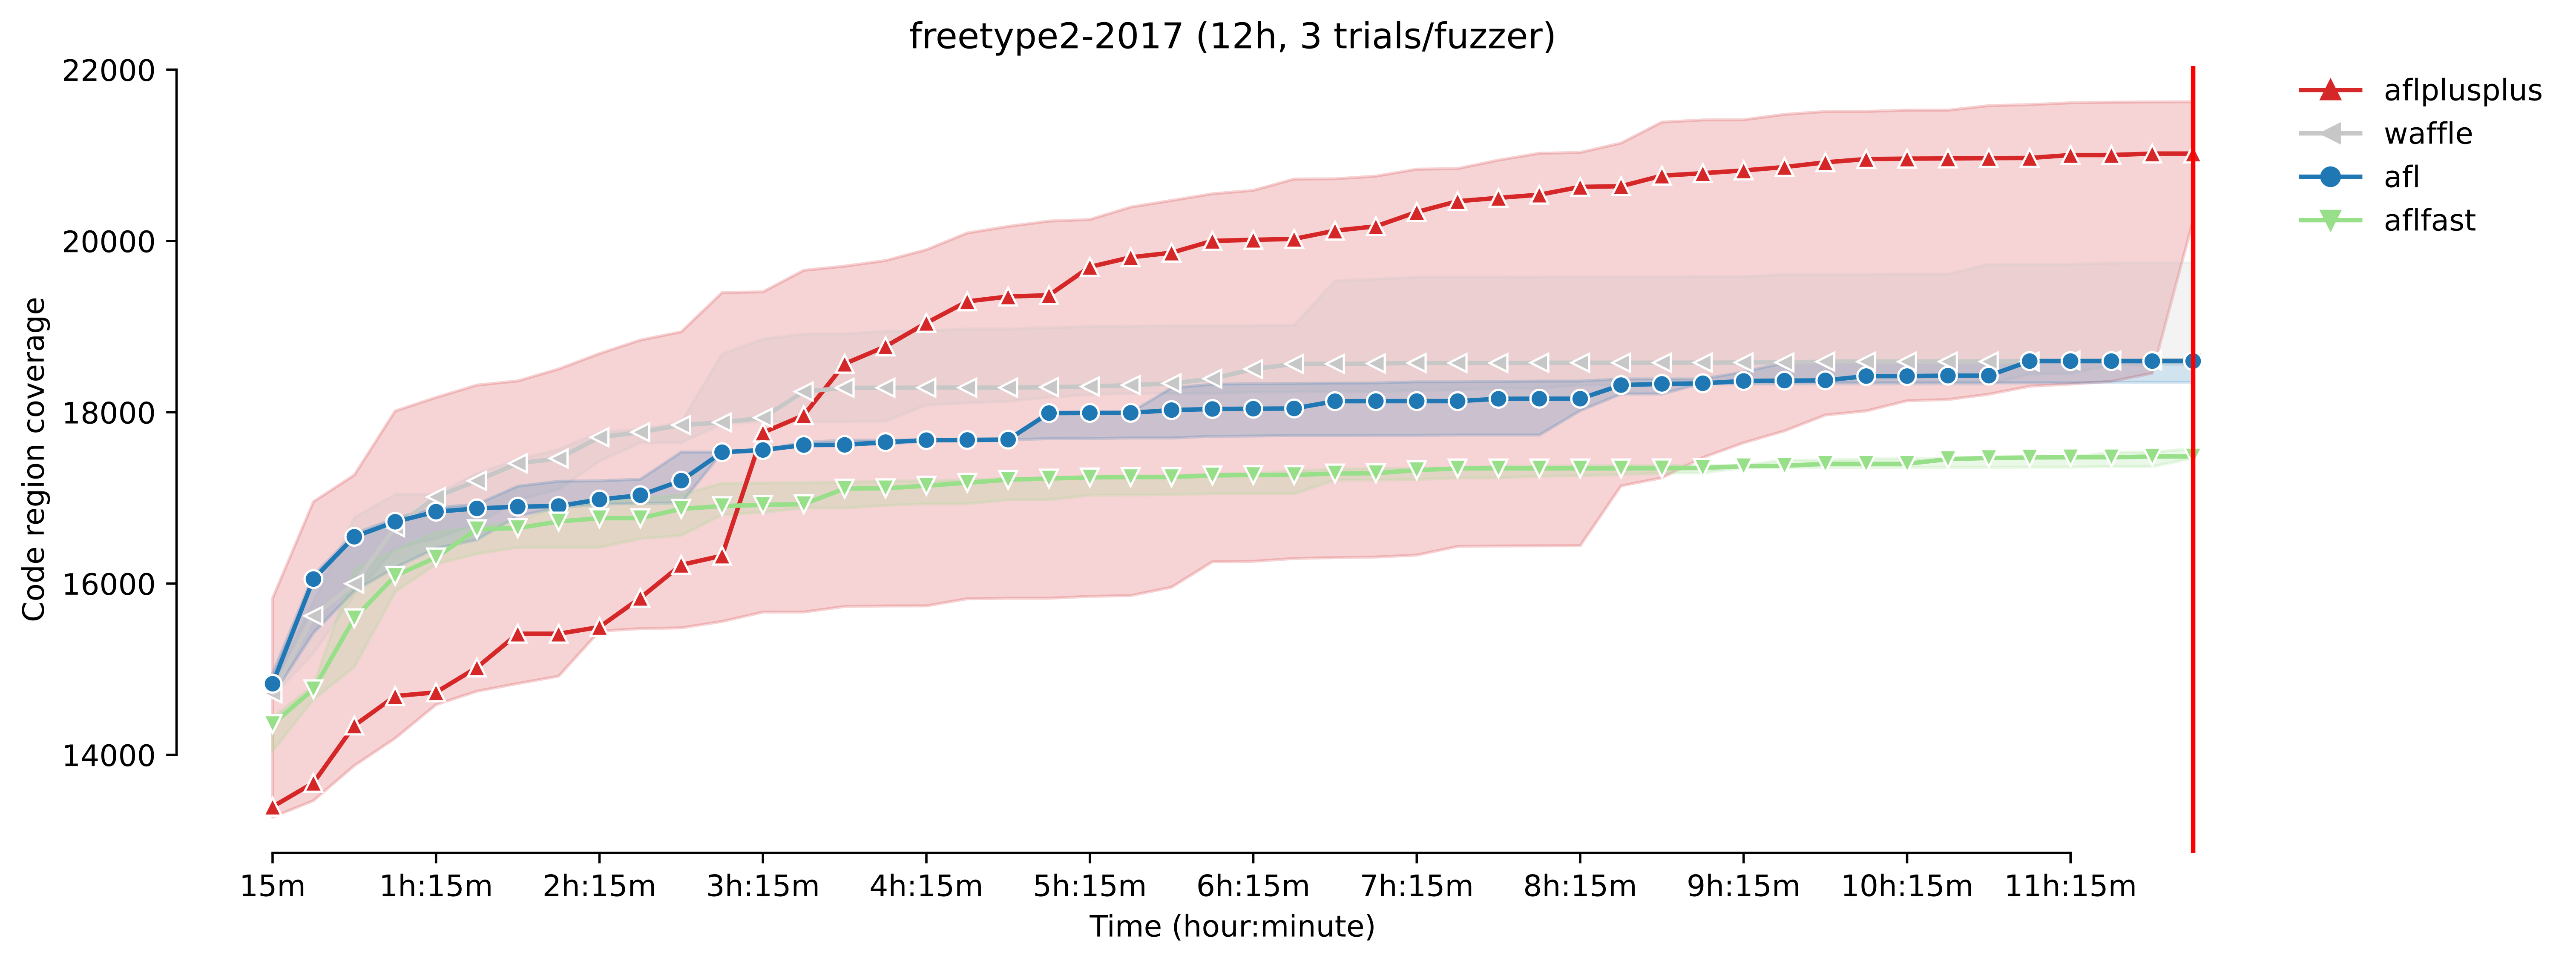
\includegraphics[width=0.85\textwidth]{Experiments/freetype2-2017_coverage_growth.png}
        \caption{freetype2-2017}
        \label{fig:sub:freetype-cov-growth}
    \end{subfigure}

    \begin{subfigure}[t]{\textwidth}
        \centering
        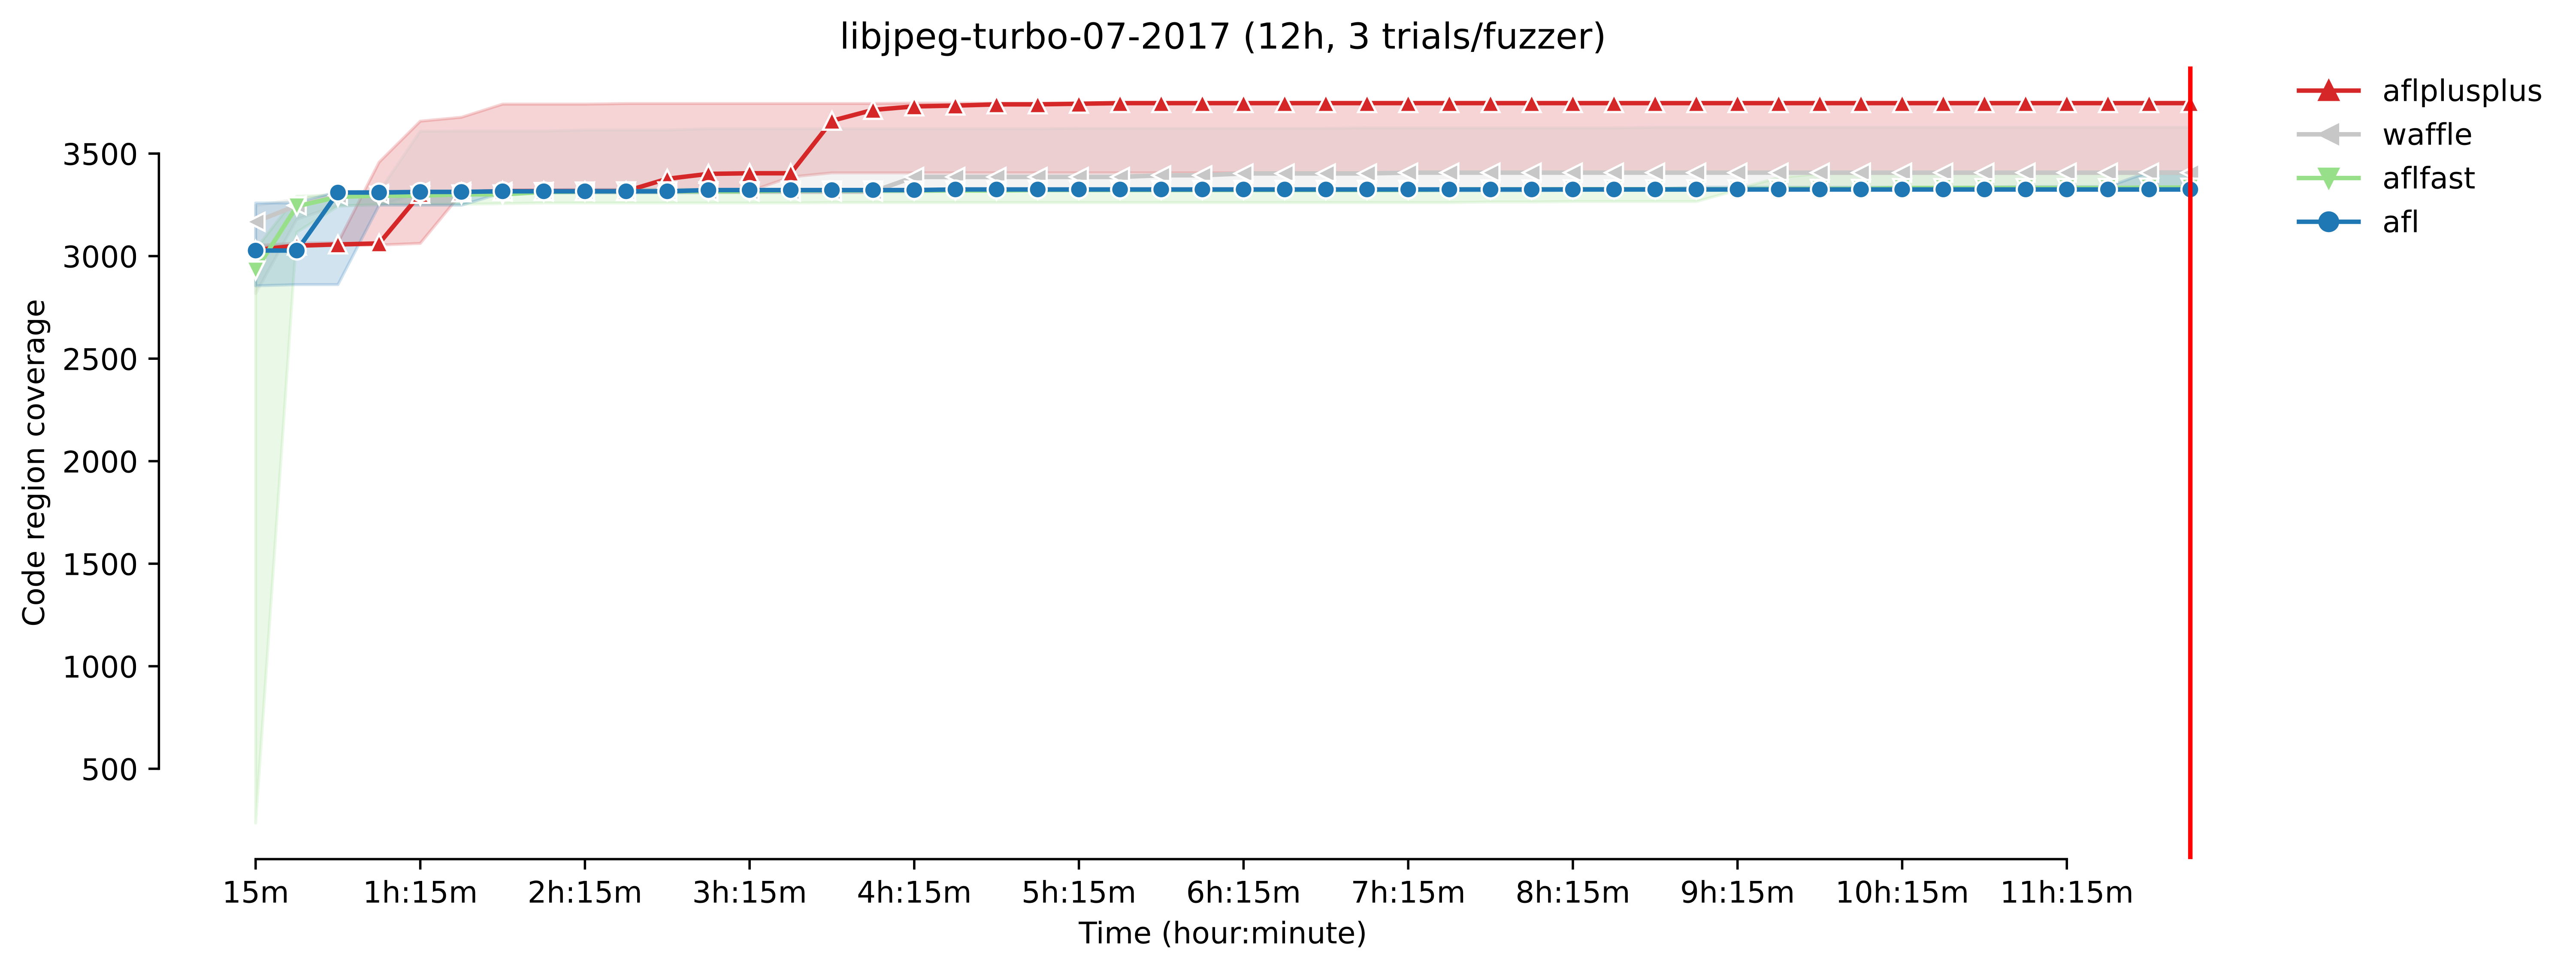
\includegraphics[width=0.85\textwidth]{Experiments/libjpeg-turbo-07-2017_coverage_growth.png}
        \caption{libjpeg-turbo-07-2017}
        \label{fig:sub:libjpeg-cov-growth}
    \end{subfigure}

    \begin{subfigure}[t]{\textwidth}
        \centering
        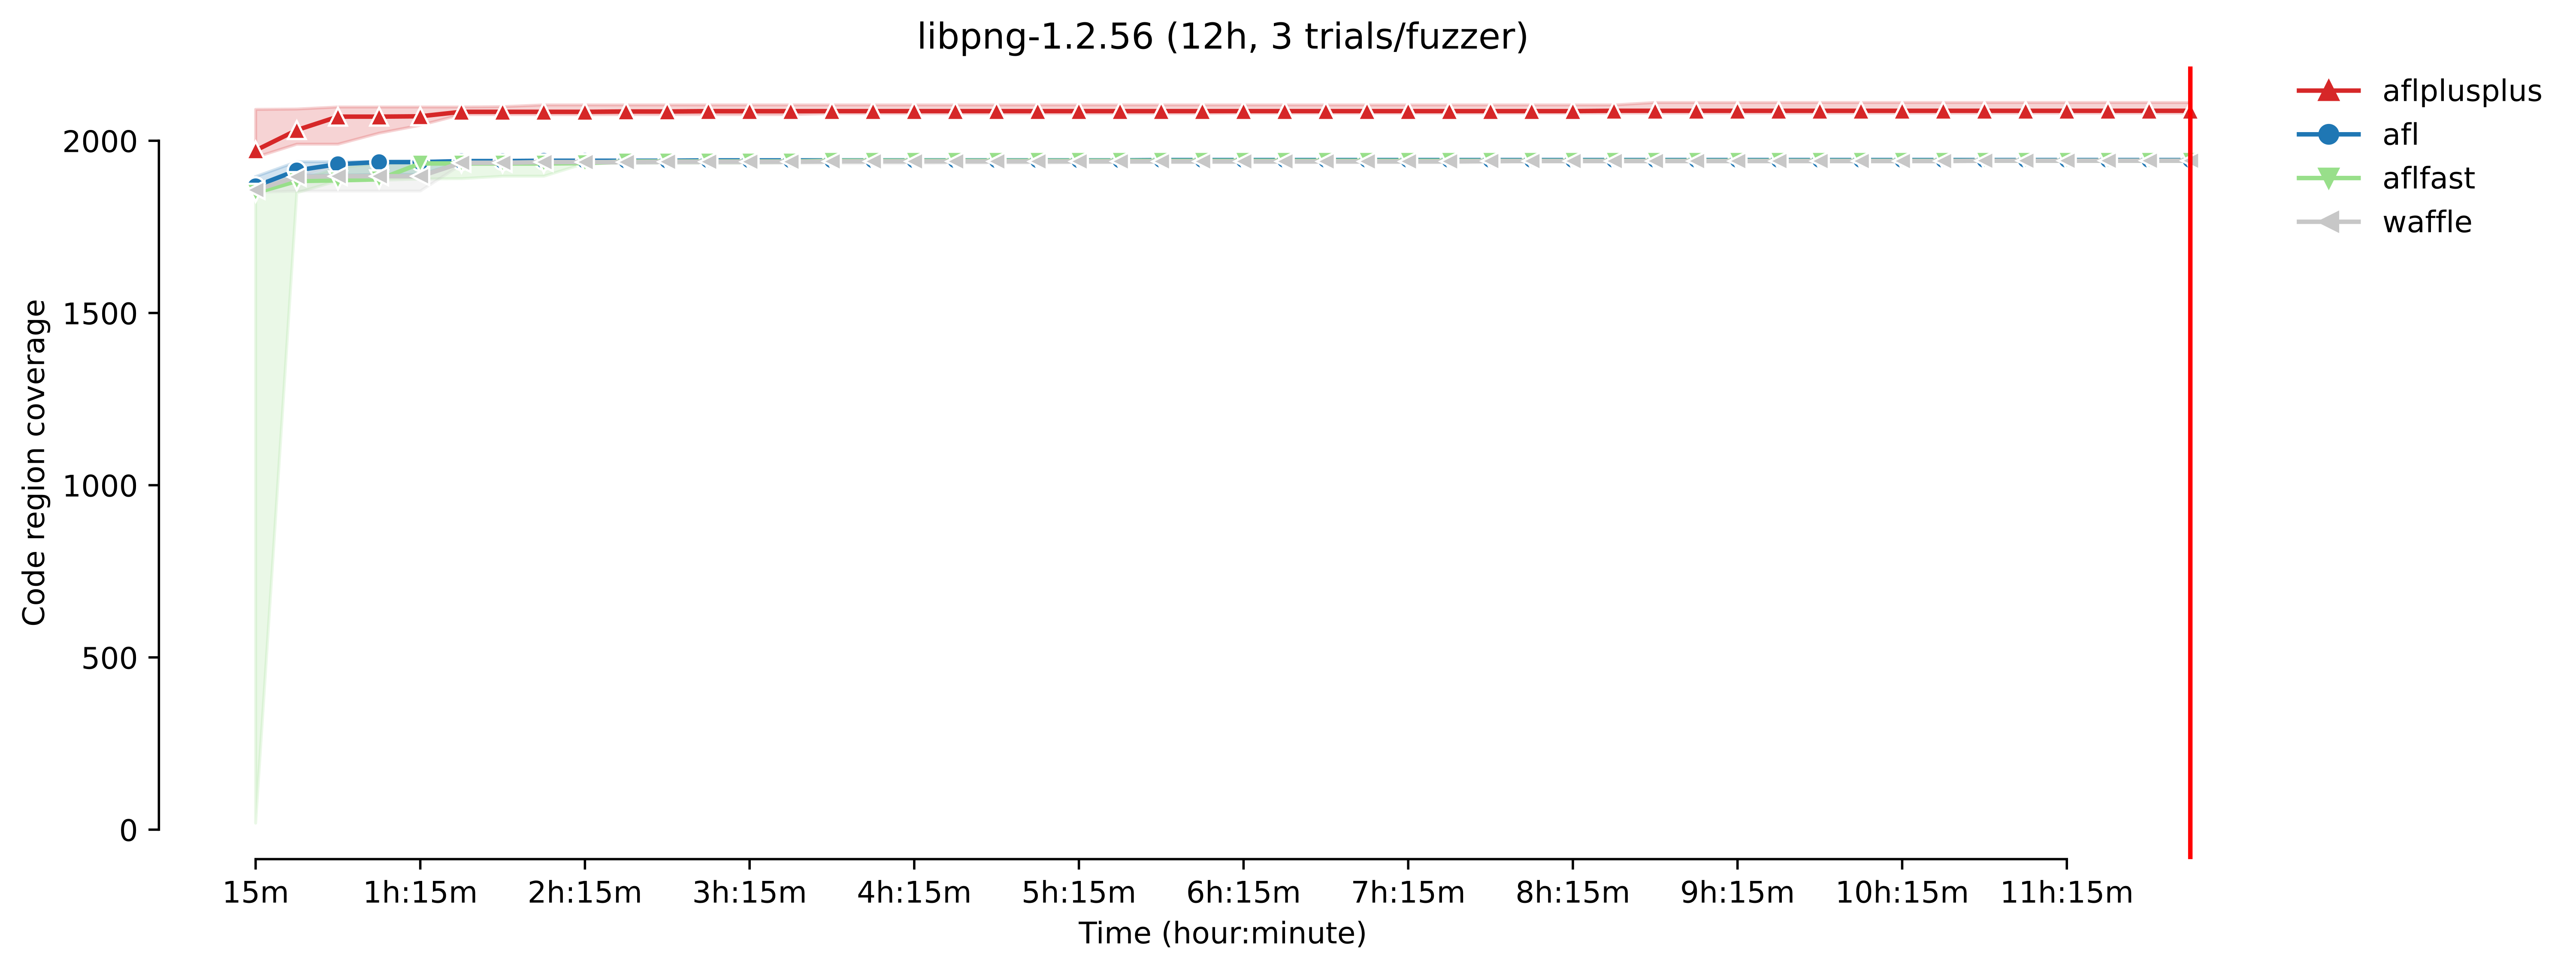
\includegraphics[width=0.85\textwidth]{Experiments/libpng-1.2.56_coverage_growth.png}
        \caption{libpng-1.2.56}
        \label{fig:sub:libpng-cov-growth}
    \end{subfigure}

    \begin{subfigure}[t]{\textwidth}
        \centering
        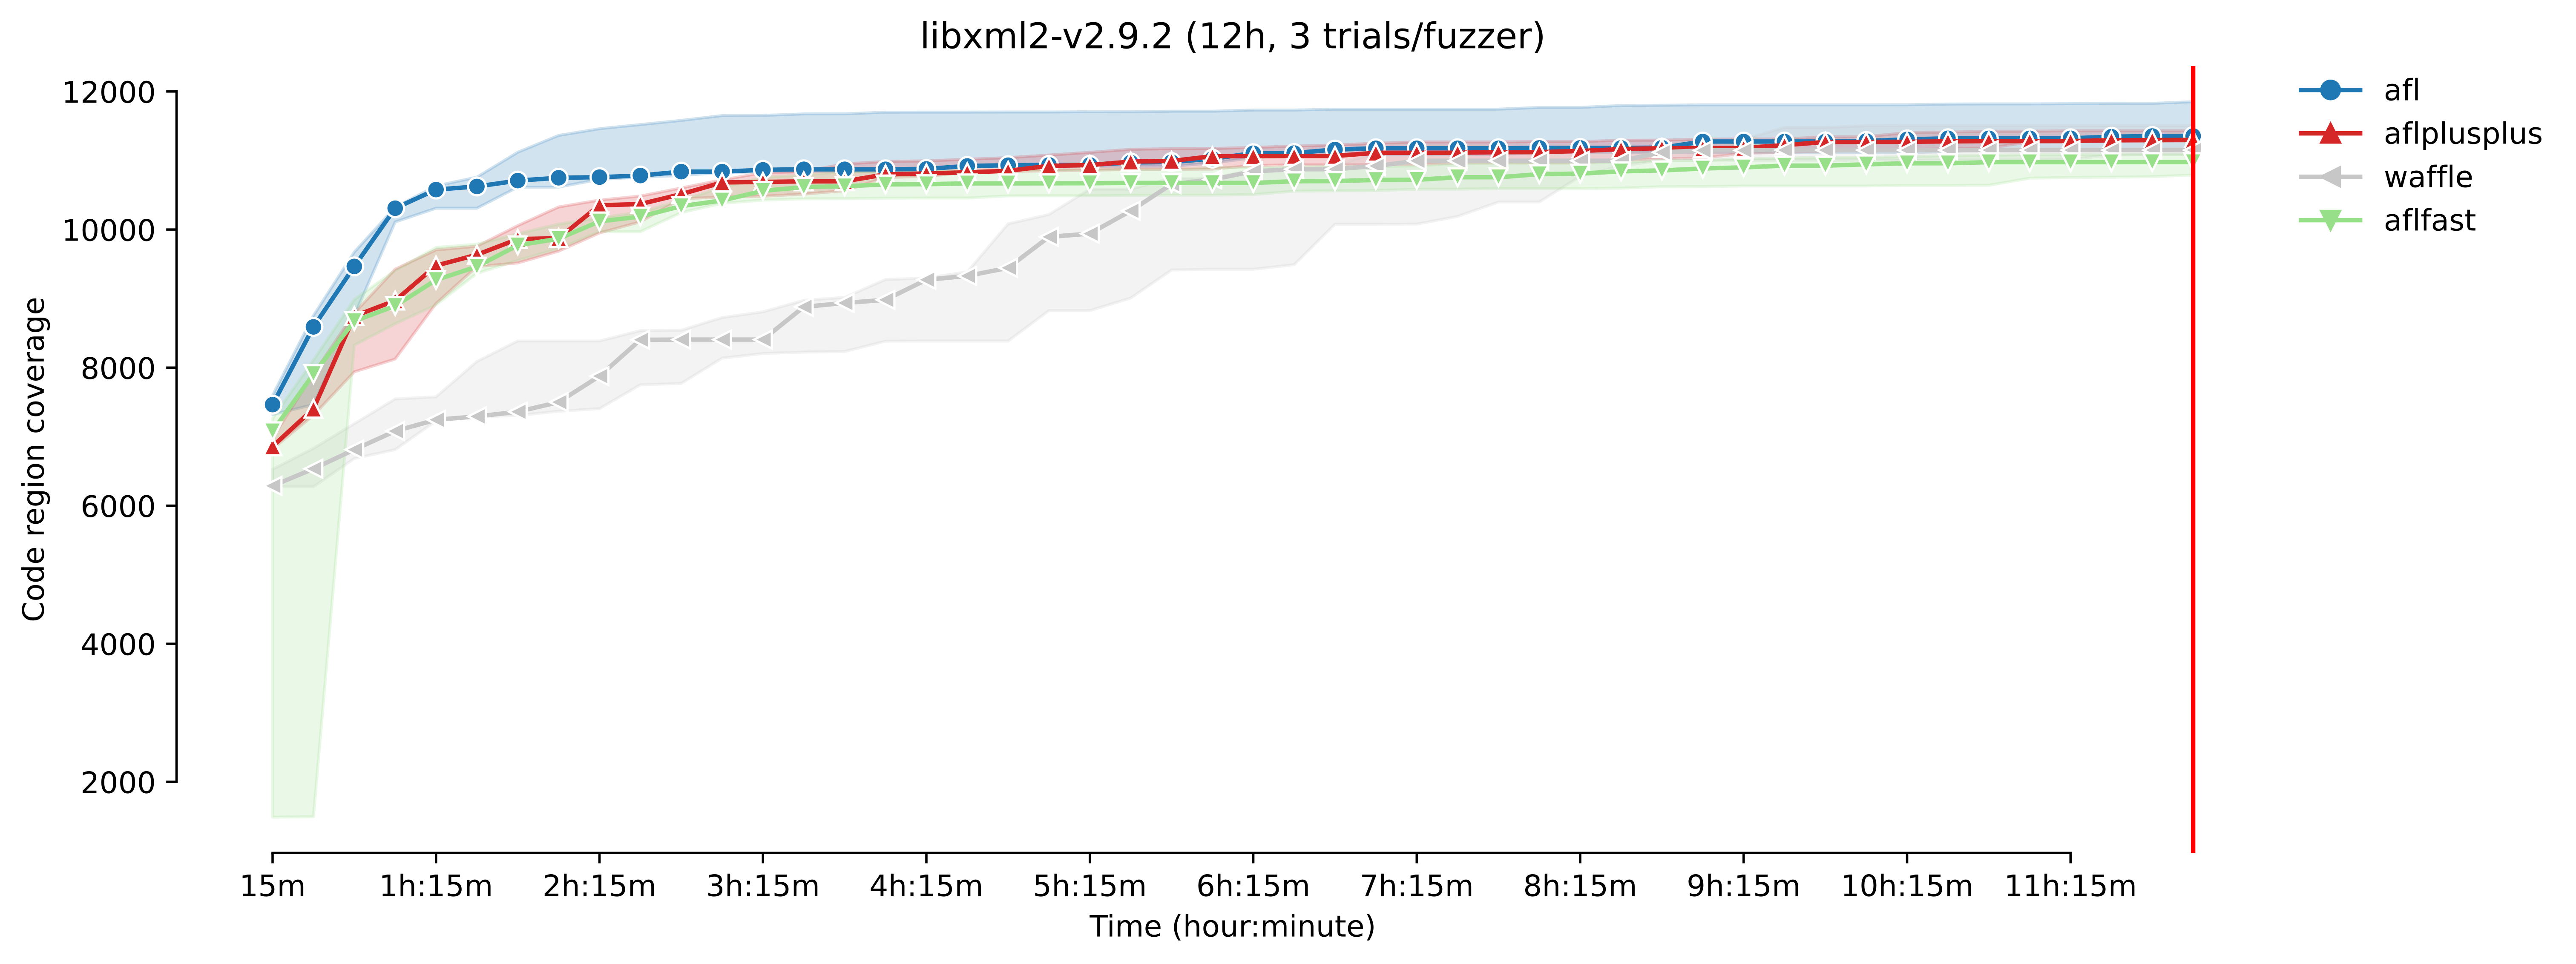
\includegraphics[width=0.85\textwidth]{Experiments/libxml2-v2.9.2_coverage_growth.png}
        \caption{libxml2-v2.9.2}
        \label{fig:sub:libxml-cov-growth}
    \end{subfigure}

    \caption{Coverage growth during the trials}
    \label{fig:cov-growth}
\end{figure}

\subsubsection{Unique code coverage findings}

Based on the results collected after each trial, fuzzbench also measures the uniqueness of the fuzzer's findings. Figure \ref{fig:cov-uniq} shows the number of code regions which were uniquely covered in a pairwise fashion. The coloring specifies the significance of the differences; the darker the color is, the more findings are uniquely found by the fuzzer on bottom.

% ! Should explain more?

\begin{figure}
    \centering
    \begin{subfigure}[t]{\textwidth}
        \centering
        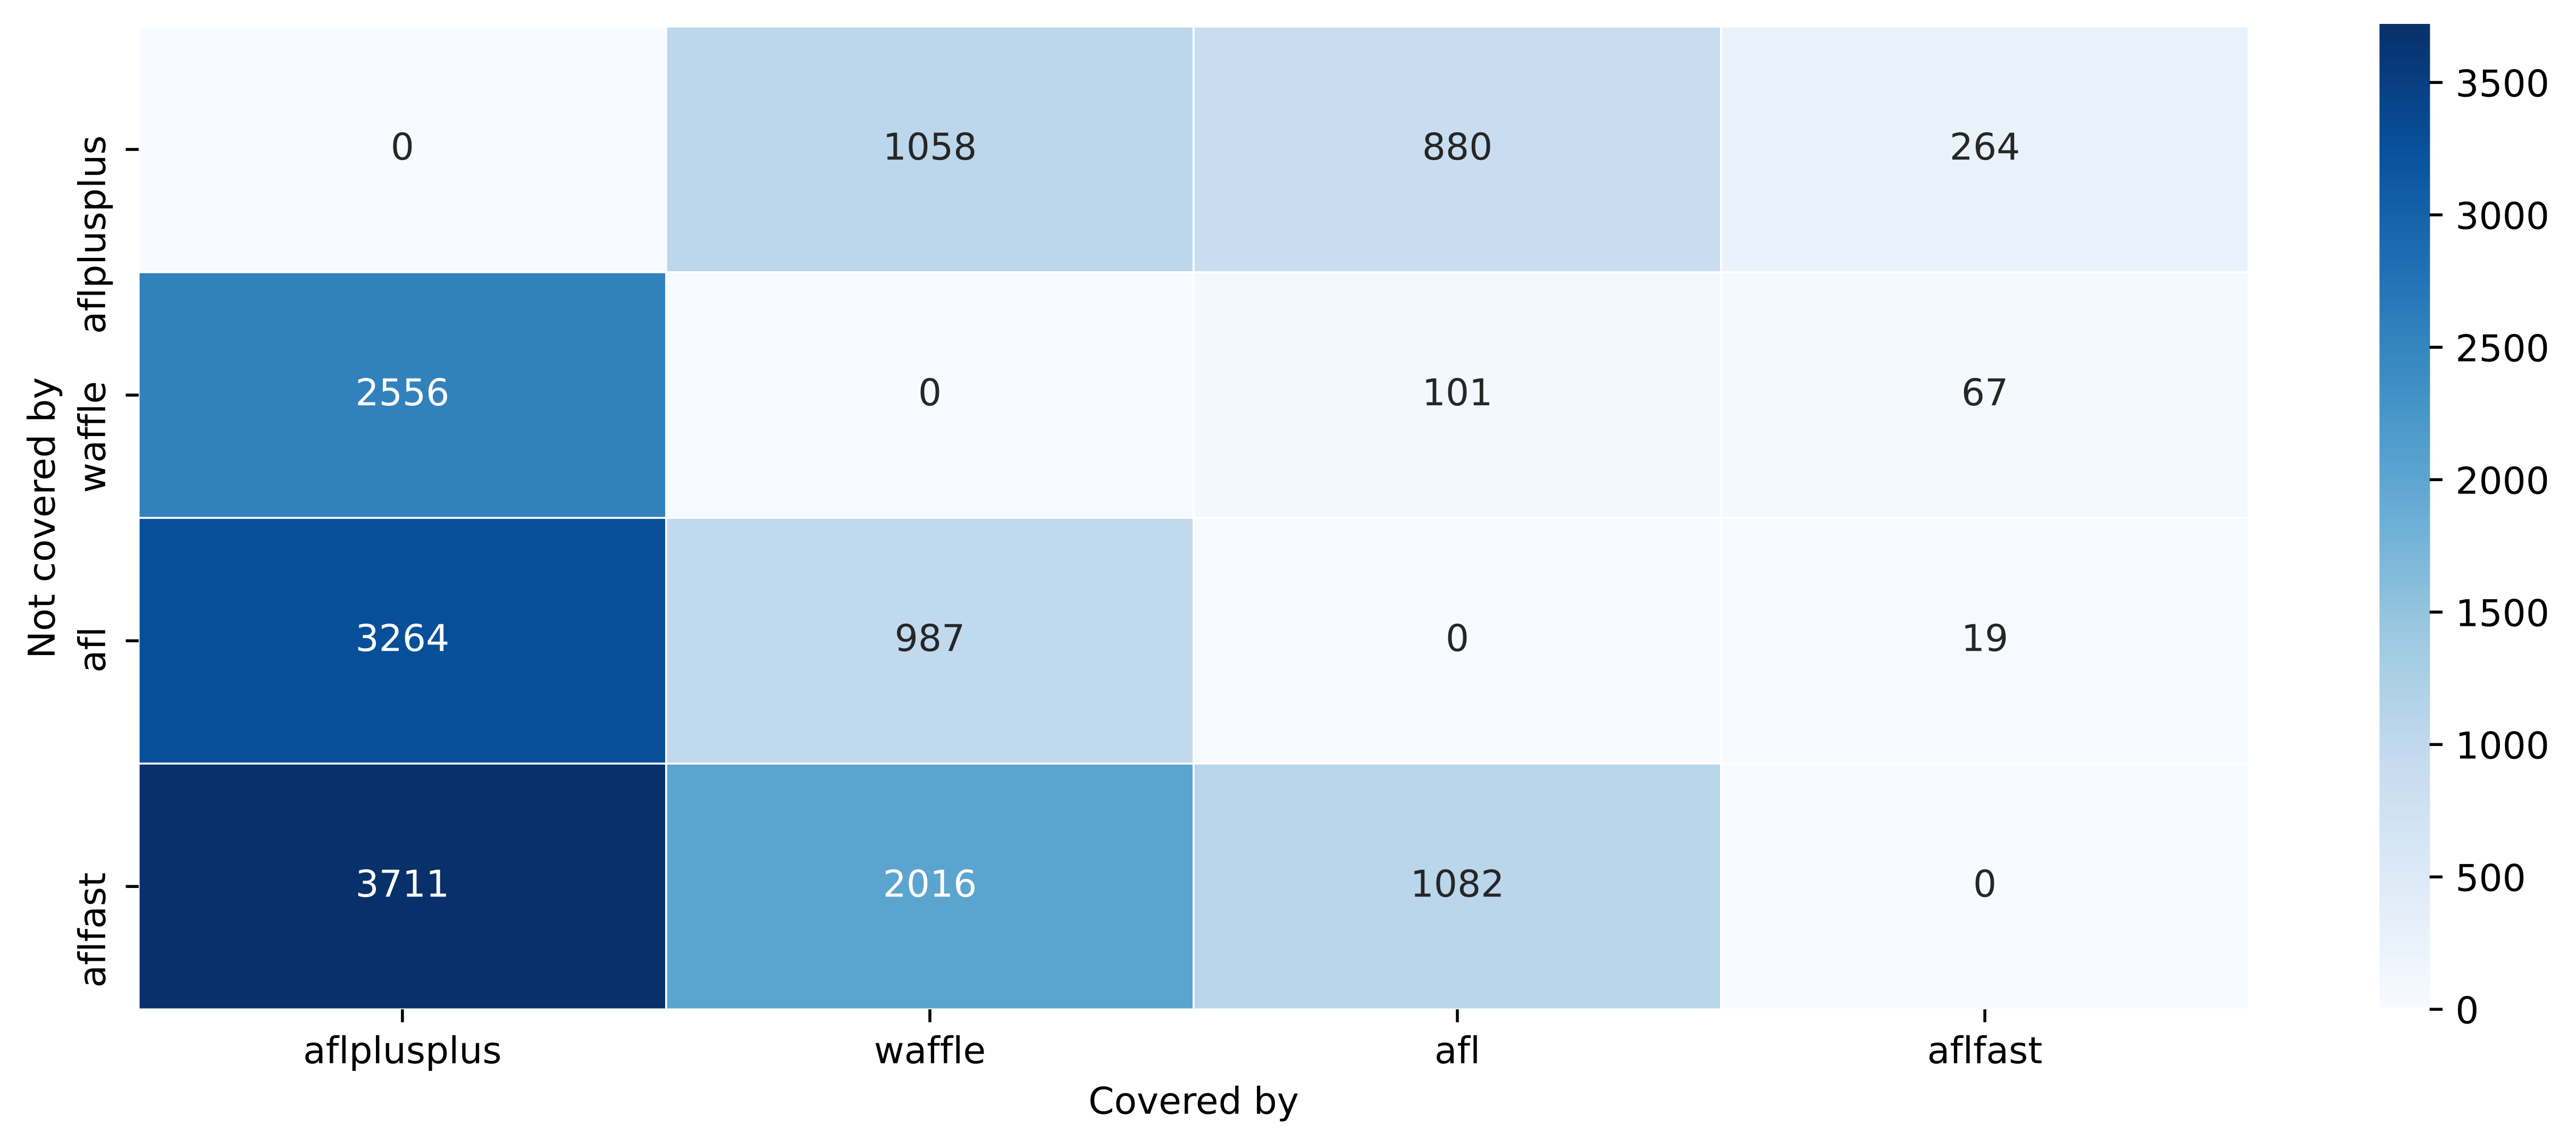
\includegraphics[width=0.70\textwidth]{Experiments/freetype2-2017_pairwise_unique_coverage_plot.png}
        \caption{freetype2-2017}
        \label{fig:sub:freetype-cov-uniq}
    \end{subfigure}

    \begin{subfigure}[t]{\textwidth}
        \centering
        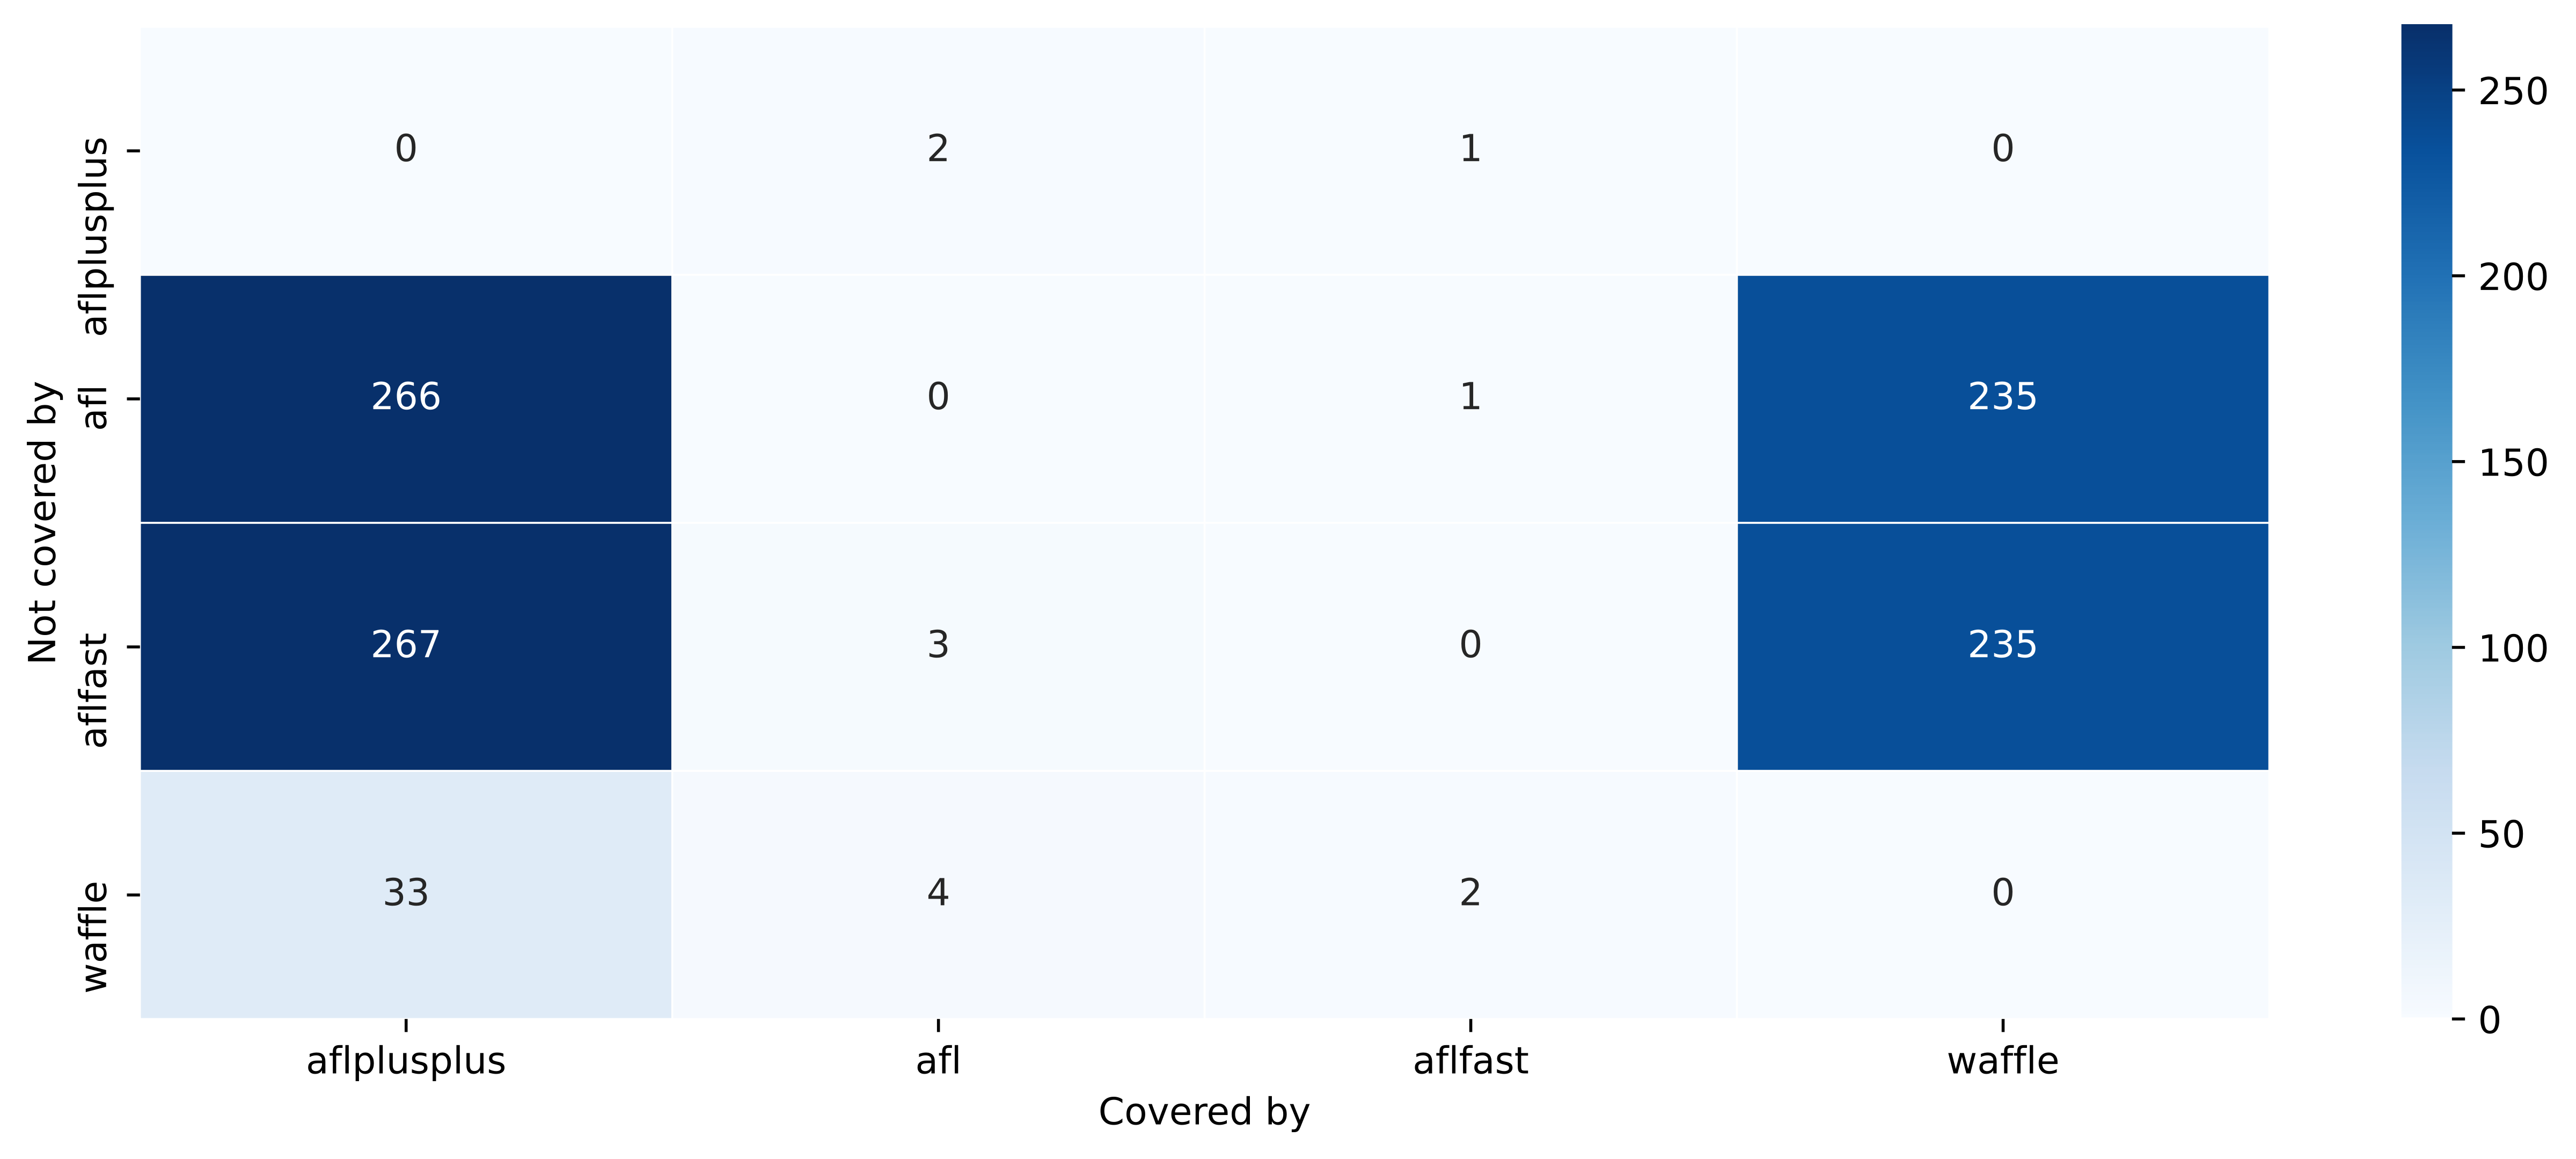
\includegraphics[width=0.70\textwidth]{Experiments/libjpeg-turbo-07-2017_pairwise_unique_coverage_plot.png}
        \caption{libjpeg-turbo-07-2017}
        \label{fig:sub:libjpeg-cov-uniq}
    \end{subfigure}

    \begin{subfigure}[t]{\textwidth}
        \centering
        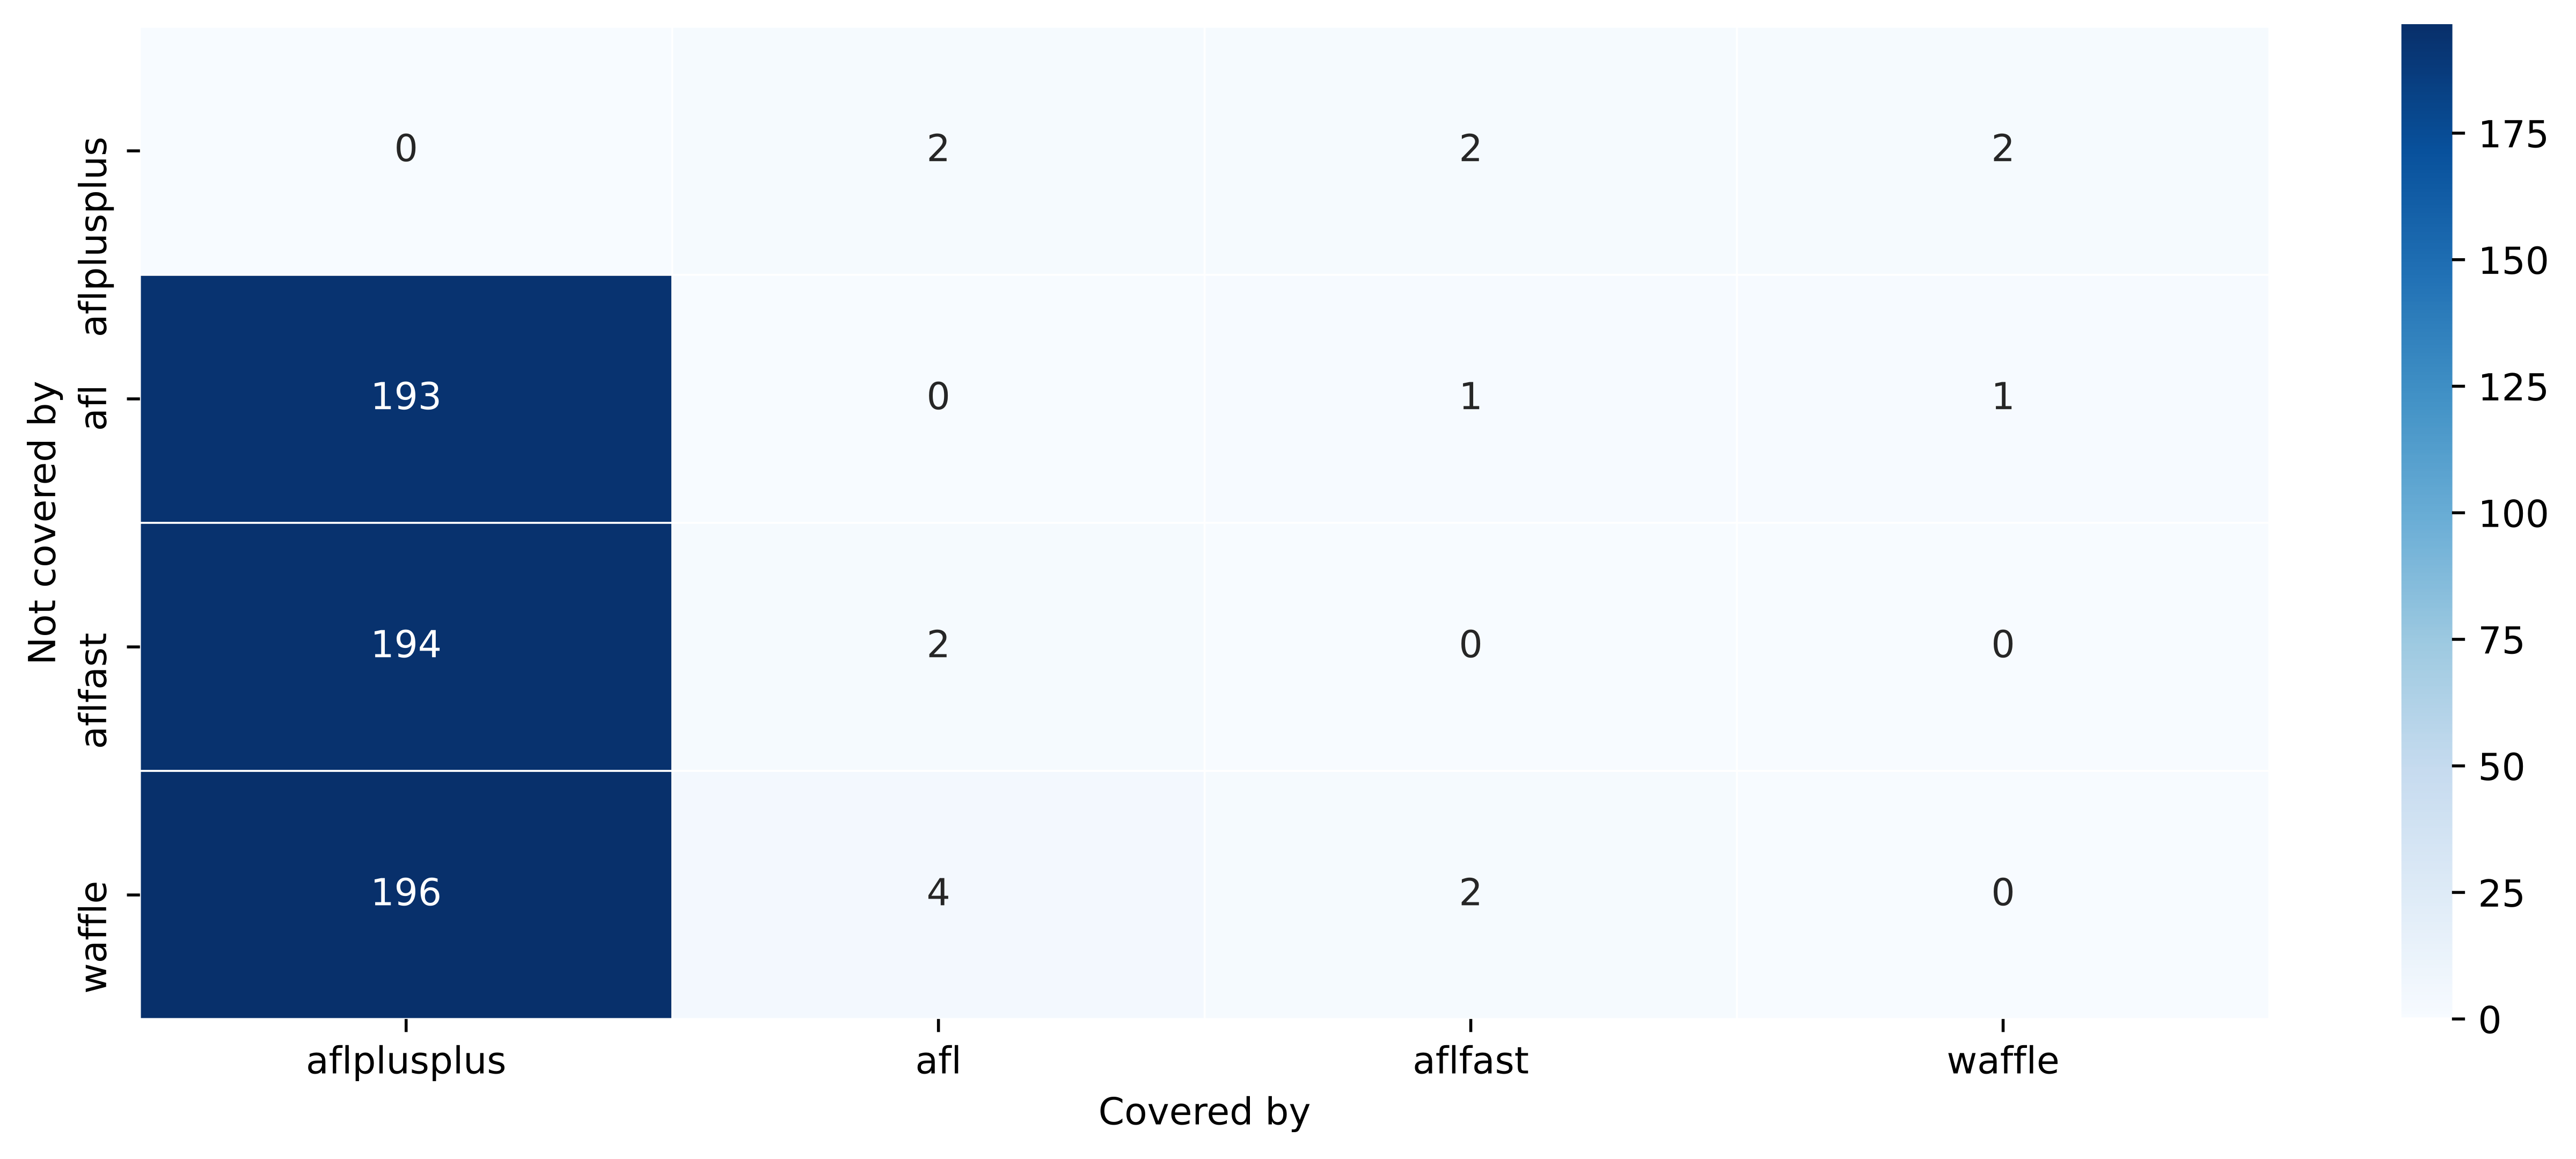
\includegraphics[width=0.70\textwidth]{Experiments/libpng-1.2.56_pairwise_unique_coverage_plot.png}
        \caption{libpng-1.2.56}
        \label{fig:sub:libpng-cov-uniq}
    \end{subfigure}

    \begin{subfigure}[t]{\textwidth}
        \centering
        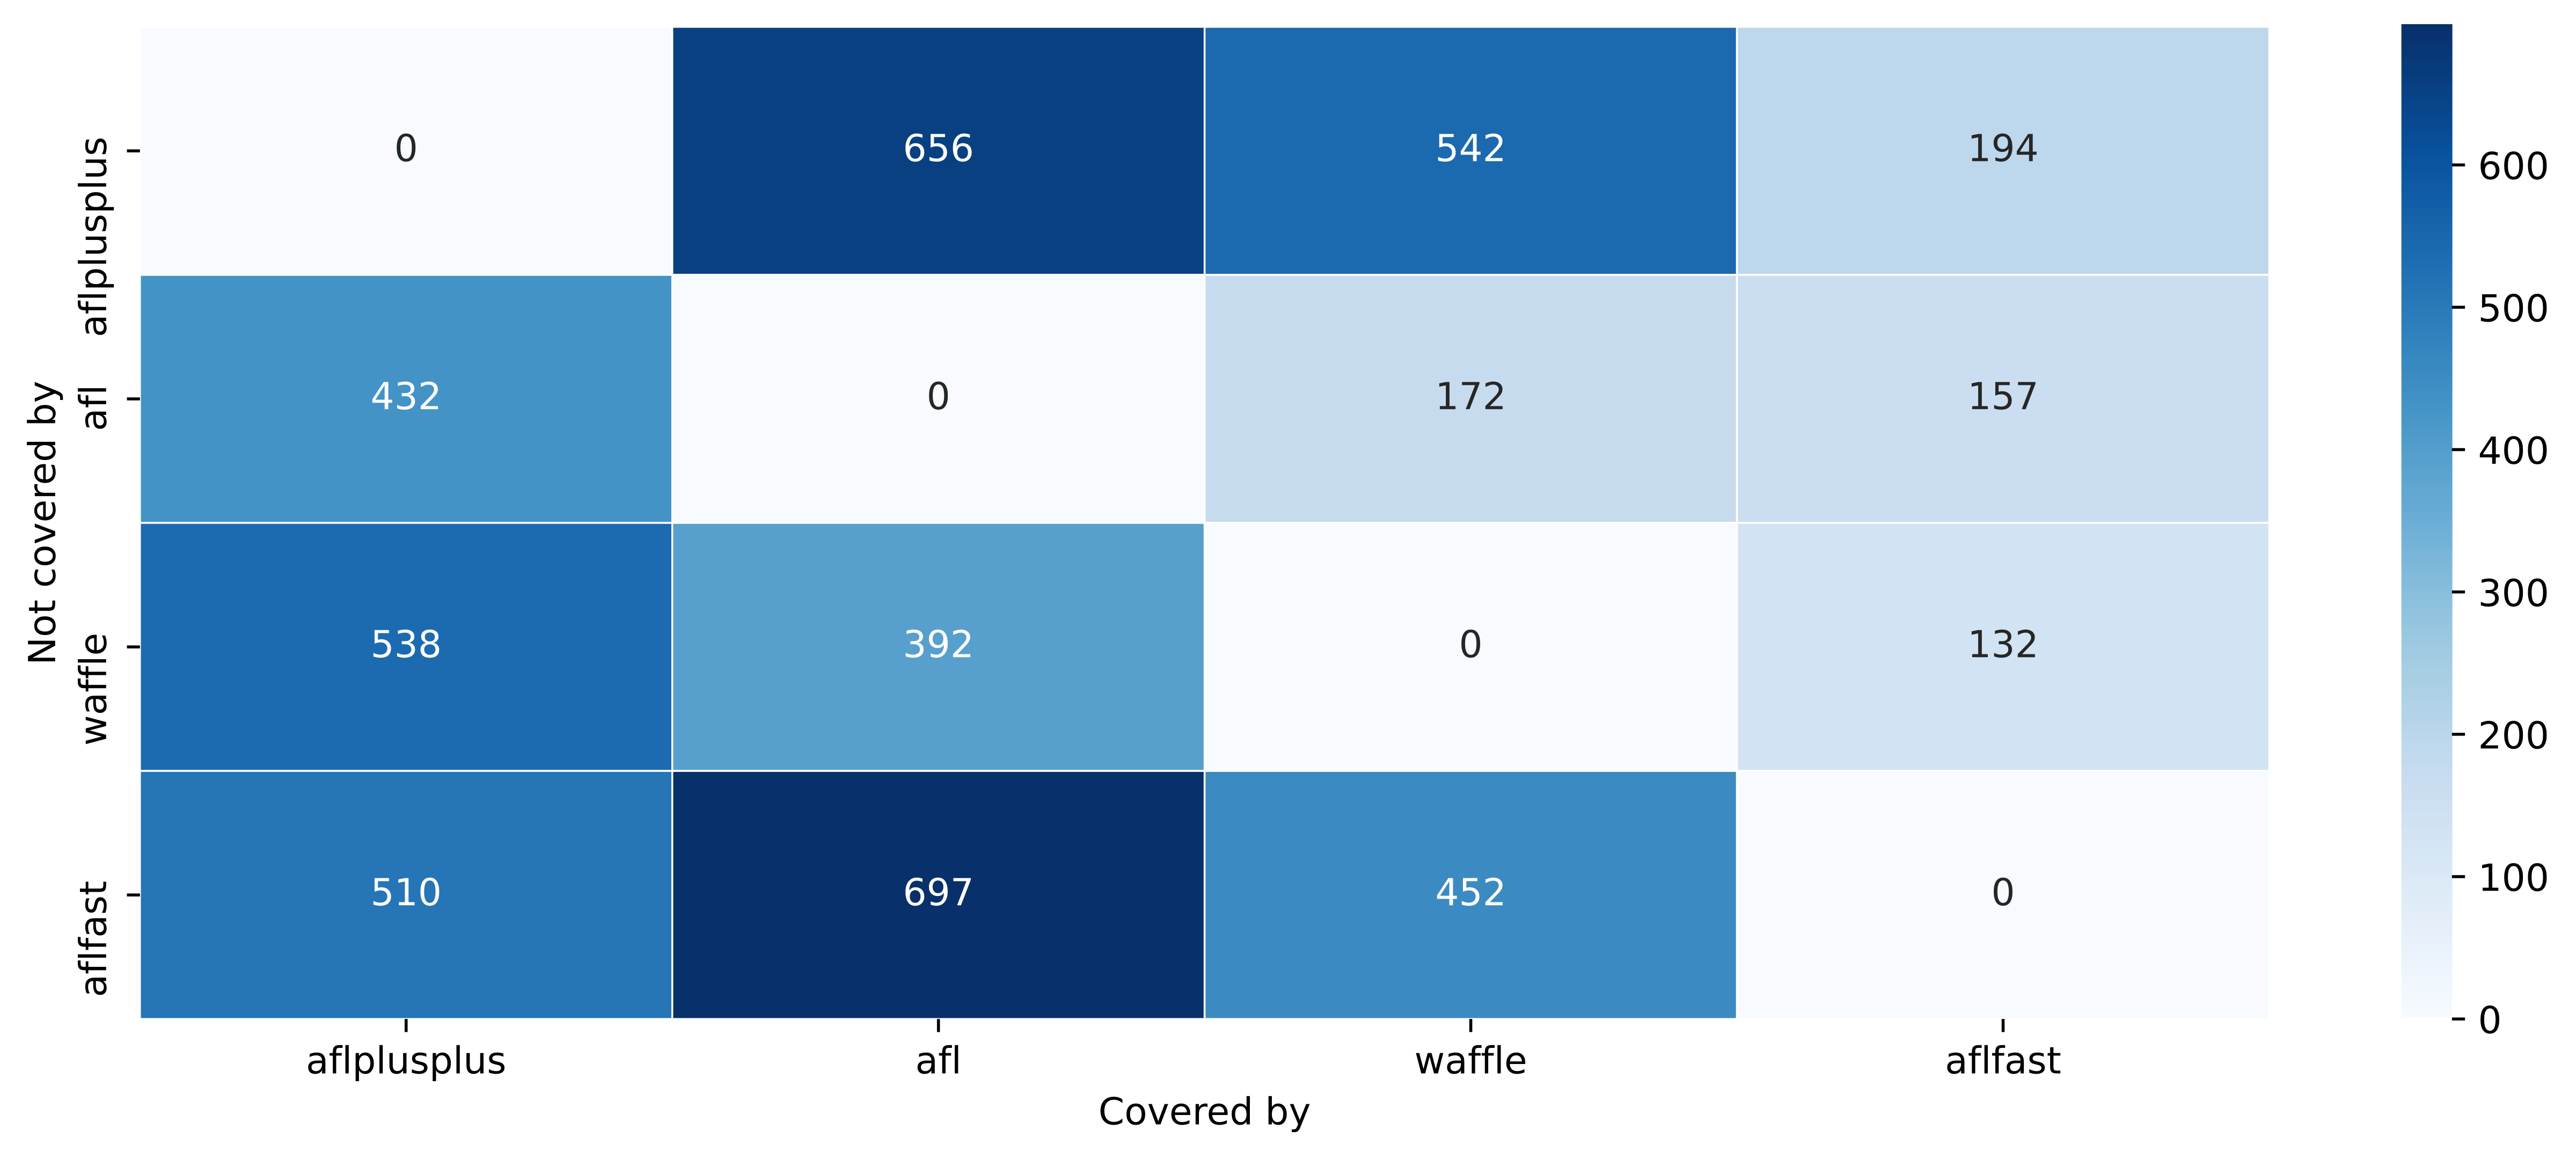
\includegraphics[width=0.70\textwidth]{Experiments/libxml2-v2.9.2_pairwise_unique_coverage_plot.png}
        \caption{libxml2-v2.9.2}
        \label{fig:sub:libxml-cov-uniq}
    \end{subfigure}

    \caption{Unique coverage findings}
    \label{fig:cov-uniq}
\end{figure}

% \subsubsection{Vargha-Delaney's A12 measurements}

% \begin{figure}
%     \centering
%     \begin{subfigure}[b]{0.475\linewidth}
%         \centering
%         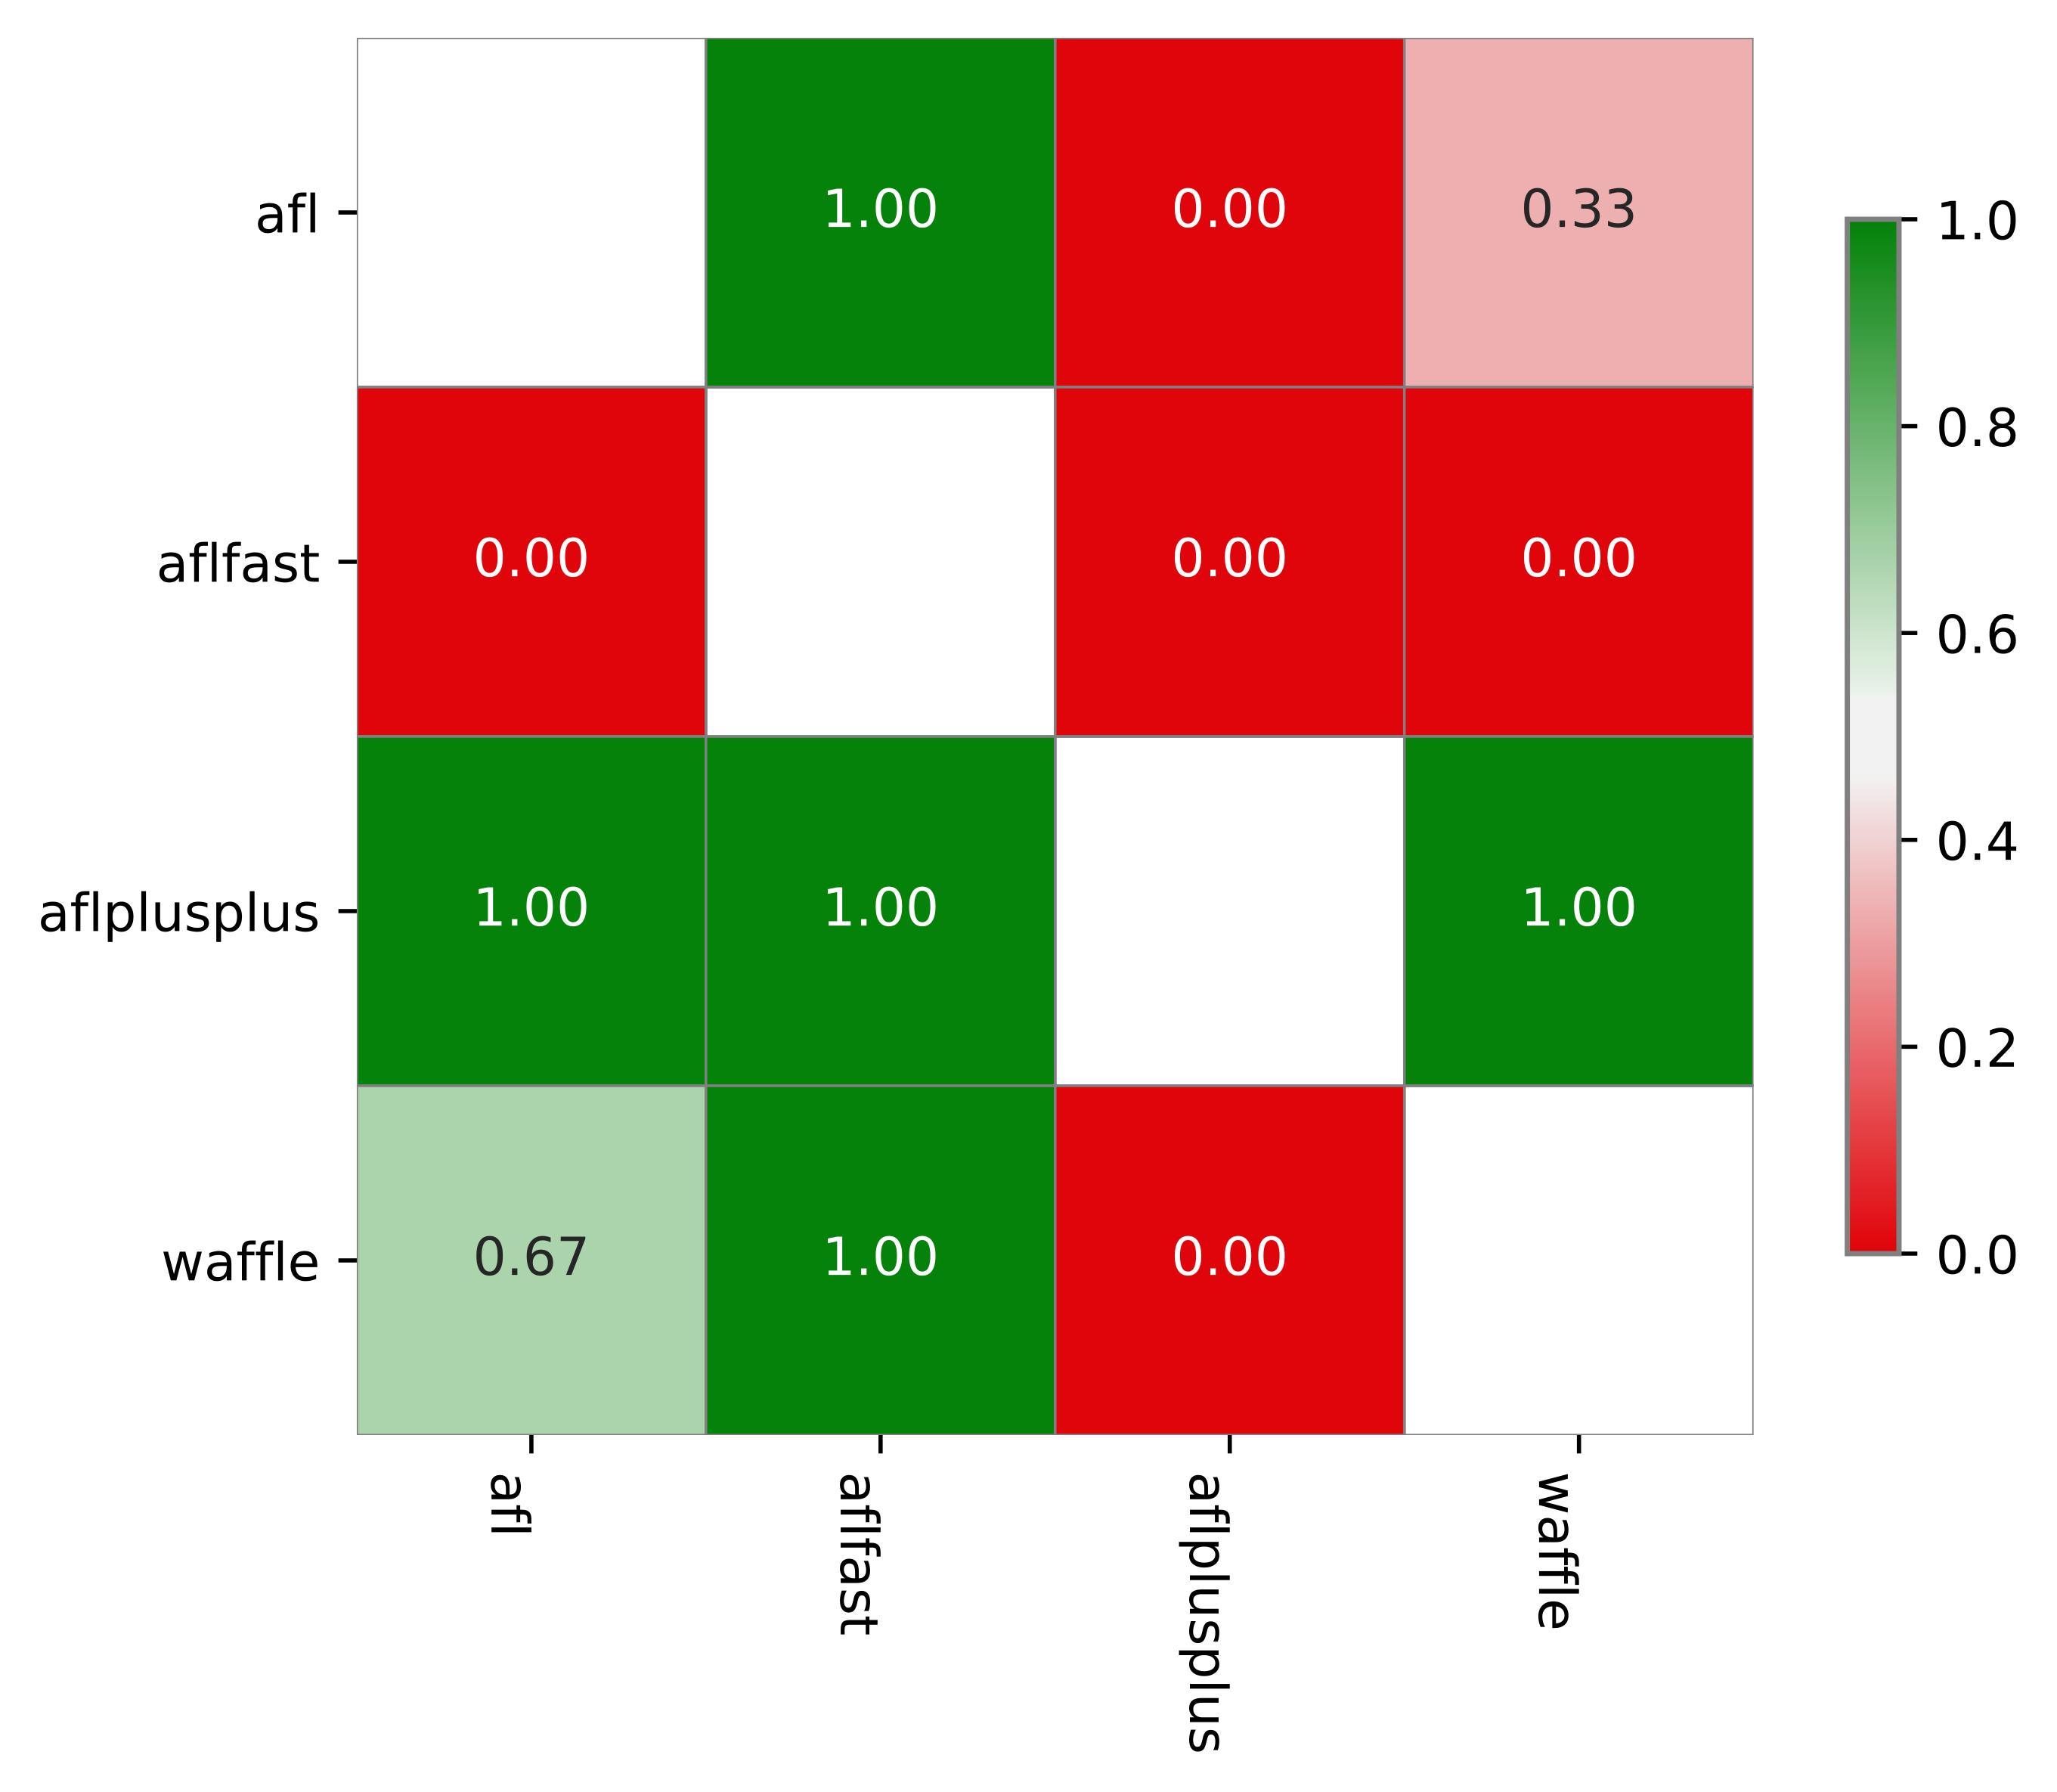
\includegraphics[width=0.95\linewidth]{Experiments/freetype2-2017_varga_delaney_a12_plot.png}
%         \caption{freetype2-2017}
%         \label{fig:sub:freetype-vda12}
%     \end{subfigure}
%     \begin{subfigure}[b]{0.475\linewidth}
%         \centering
%         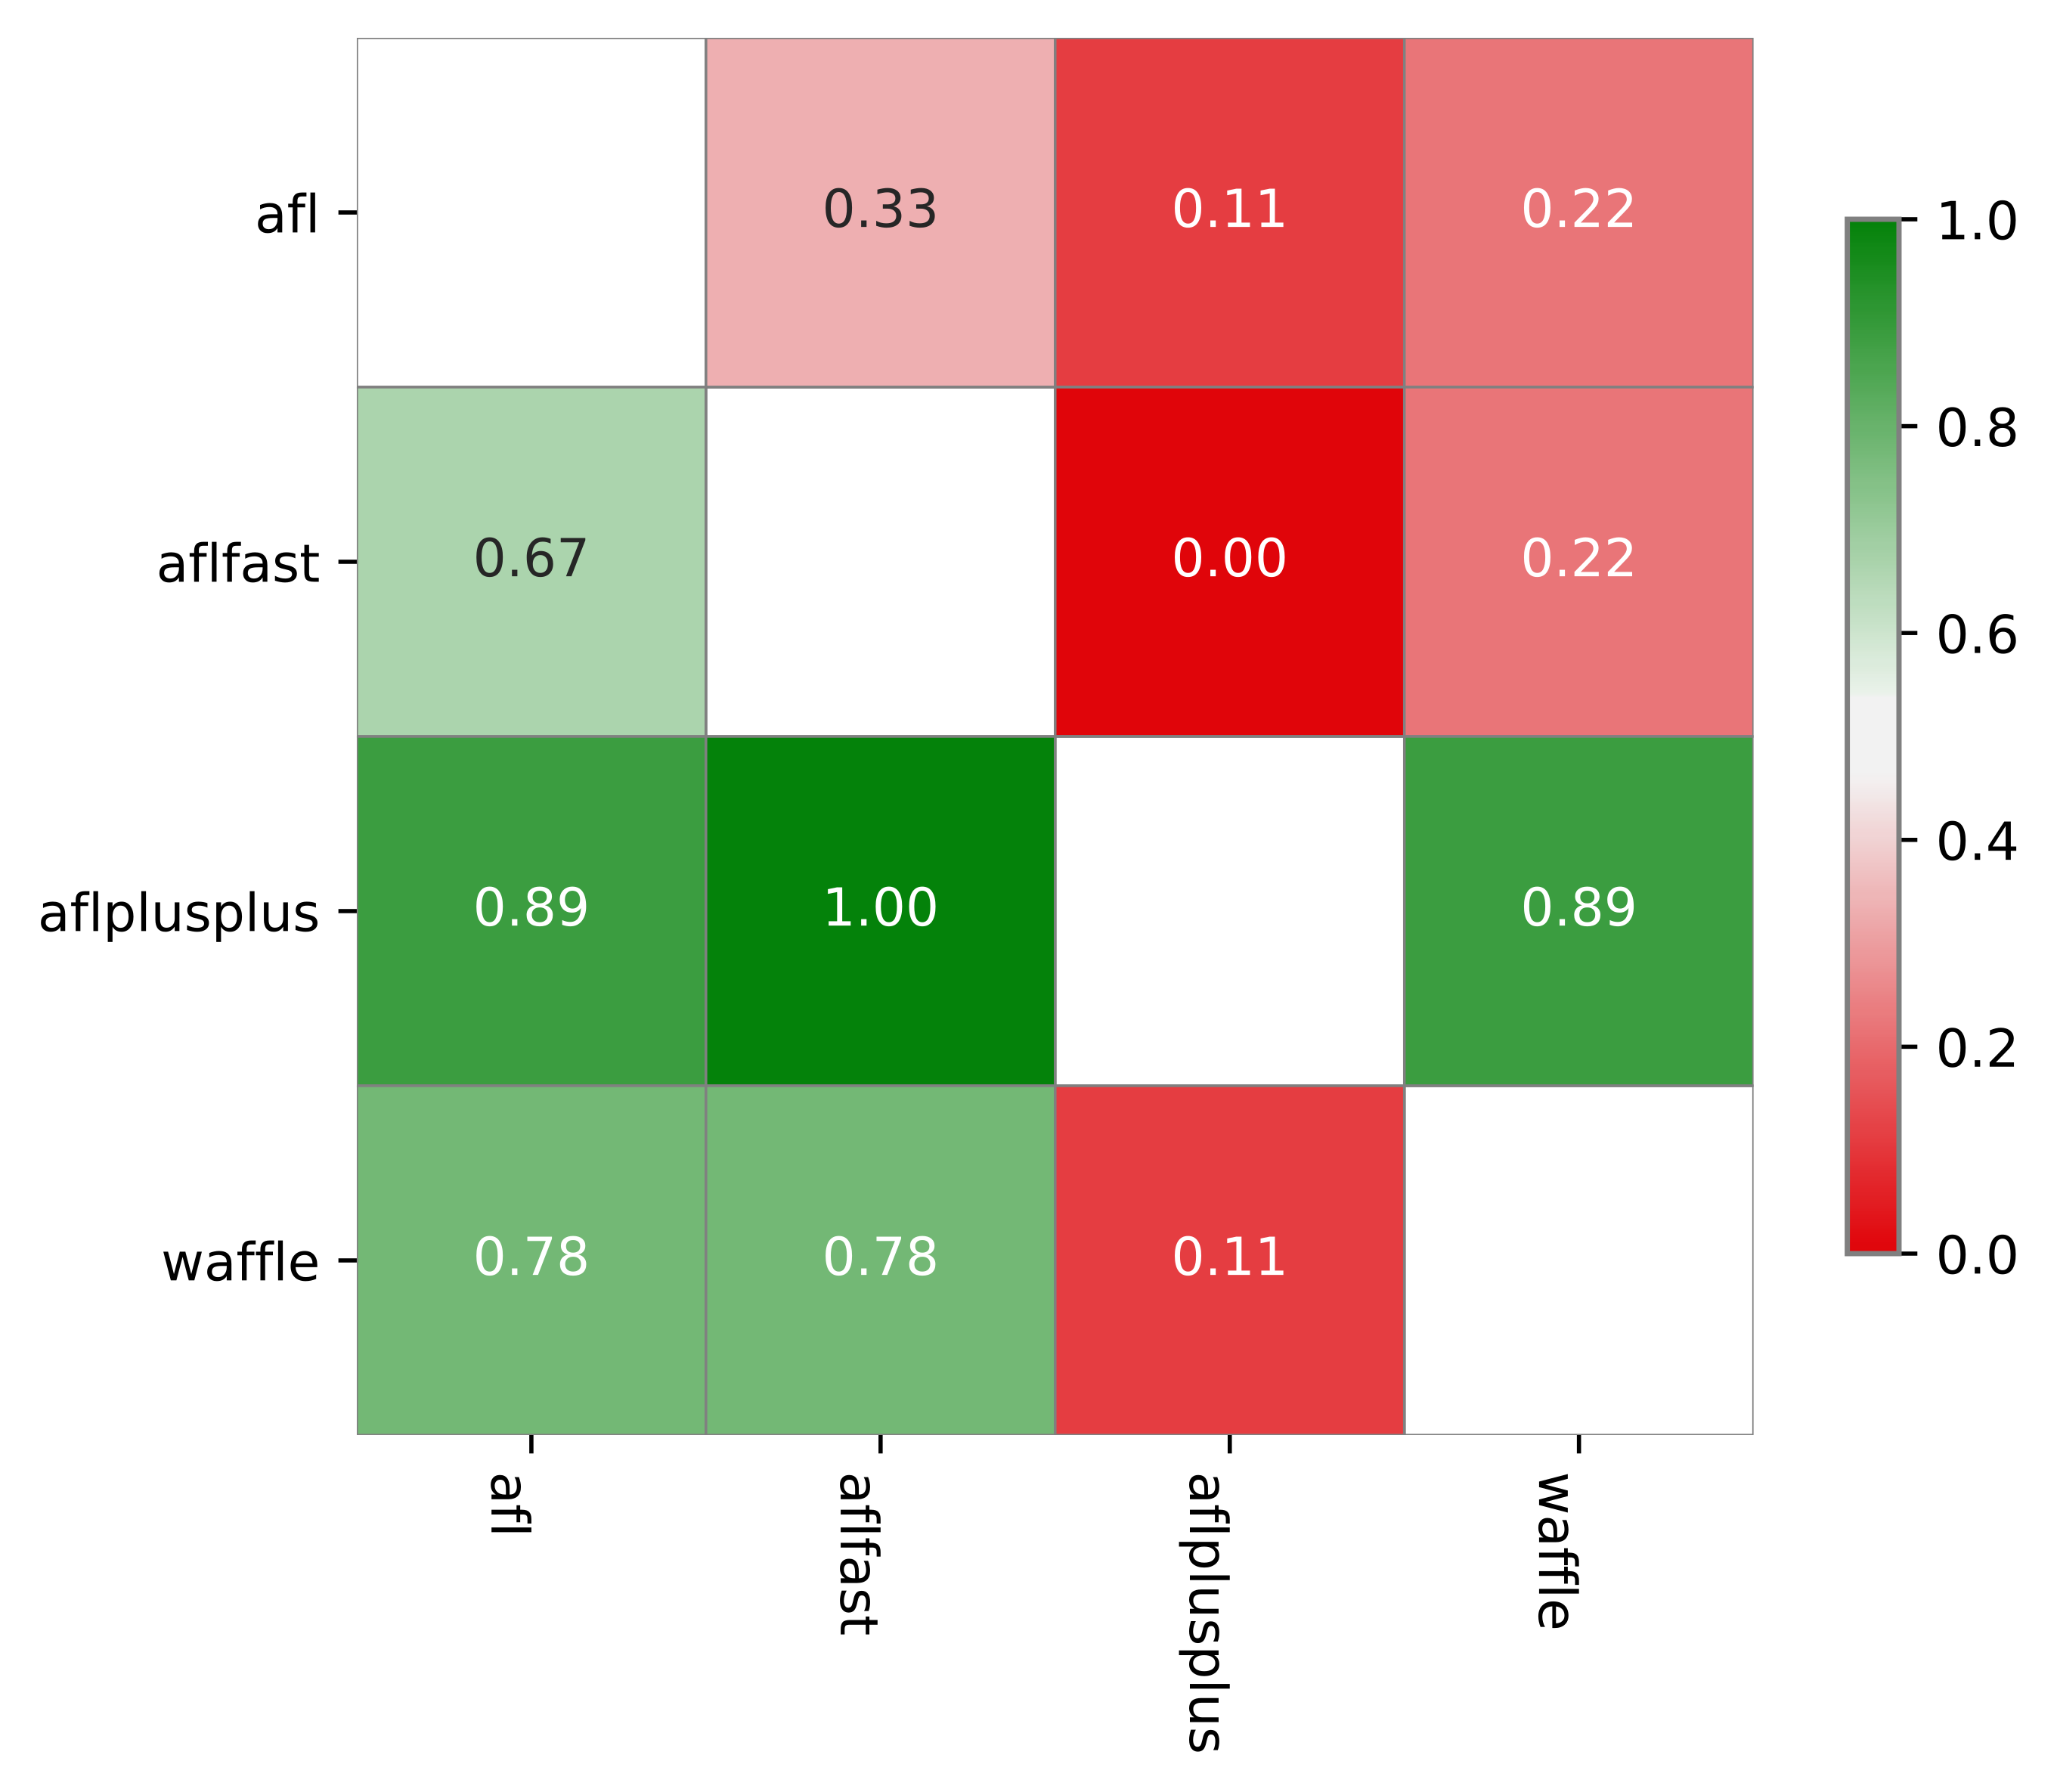
\includegraphics[width=0.95\linewidth]{Experiments/libjpeg-turbo-07-2017_varga_delaney_a12_plot.png}
%         \caption{libjpeg-turbo-07-2017}
%         \label{fig:sub:libjpeg-vda12}
%     \end{subfigure}

%     \begin{subfigure}[b]{0.475\linewidth}
%         \centering
%         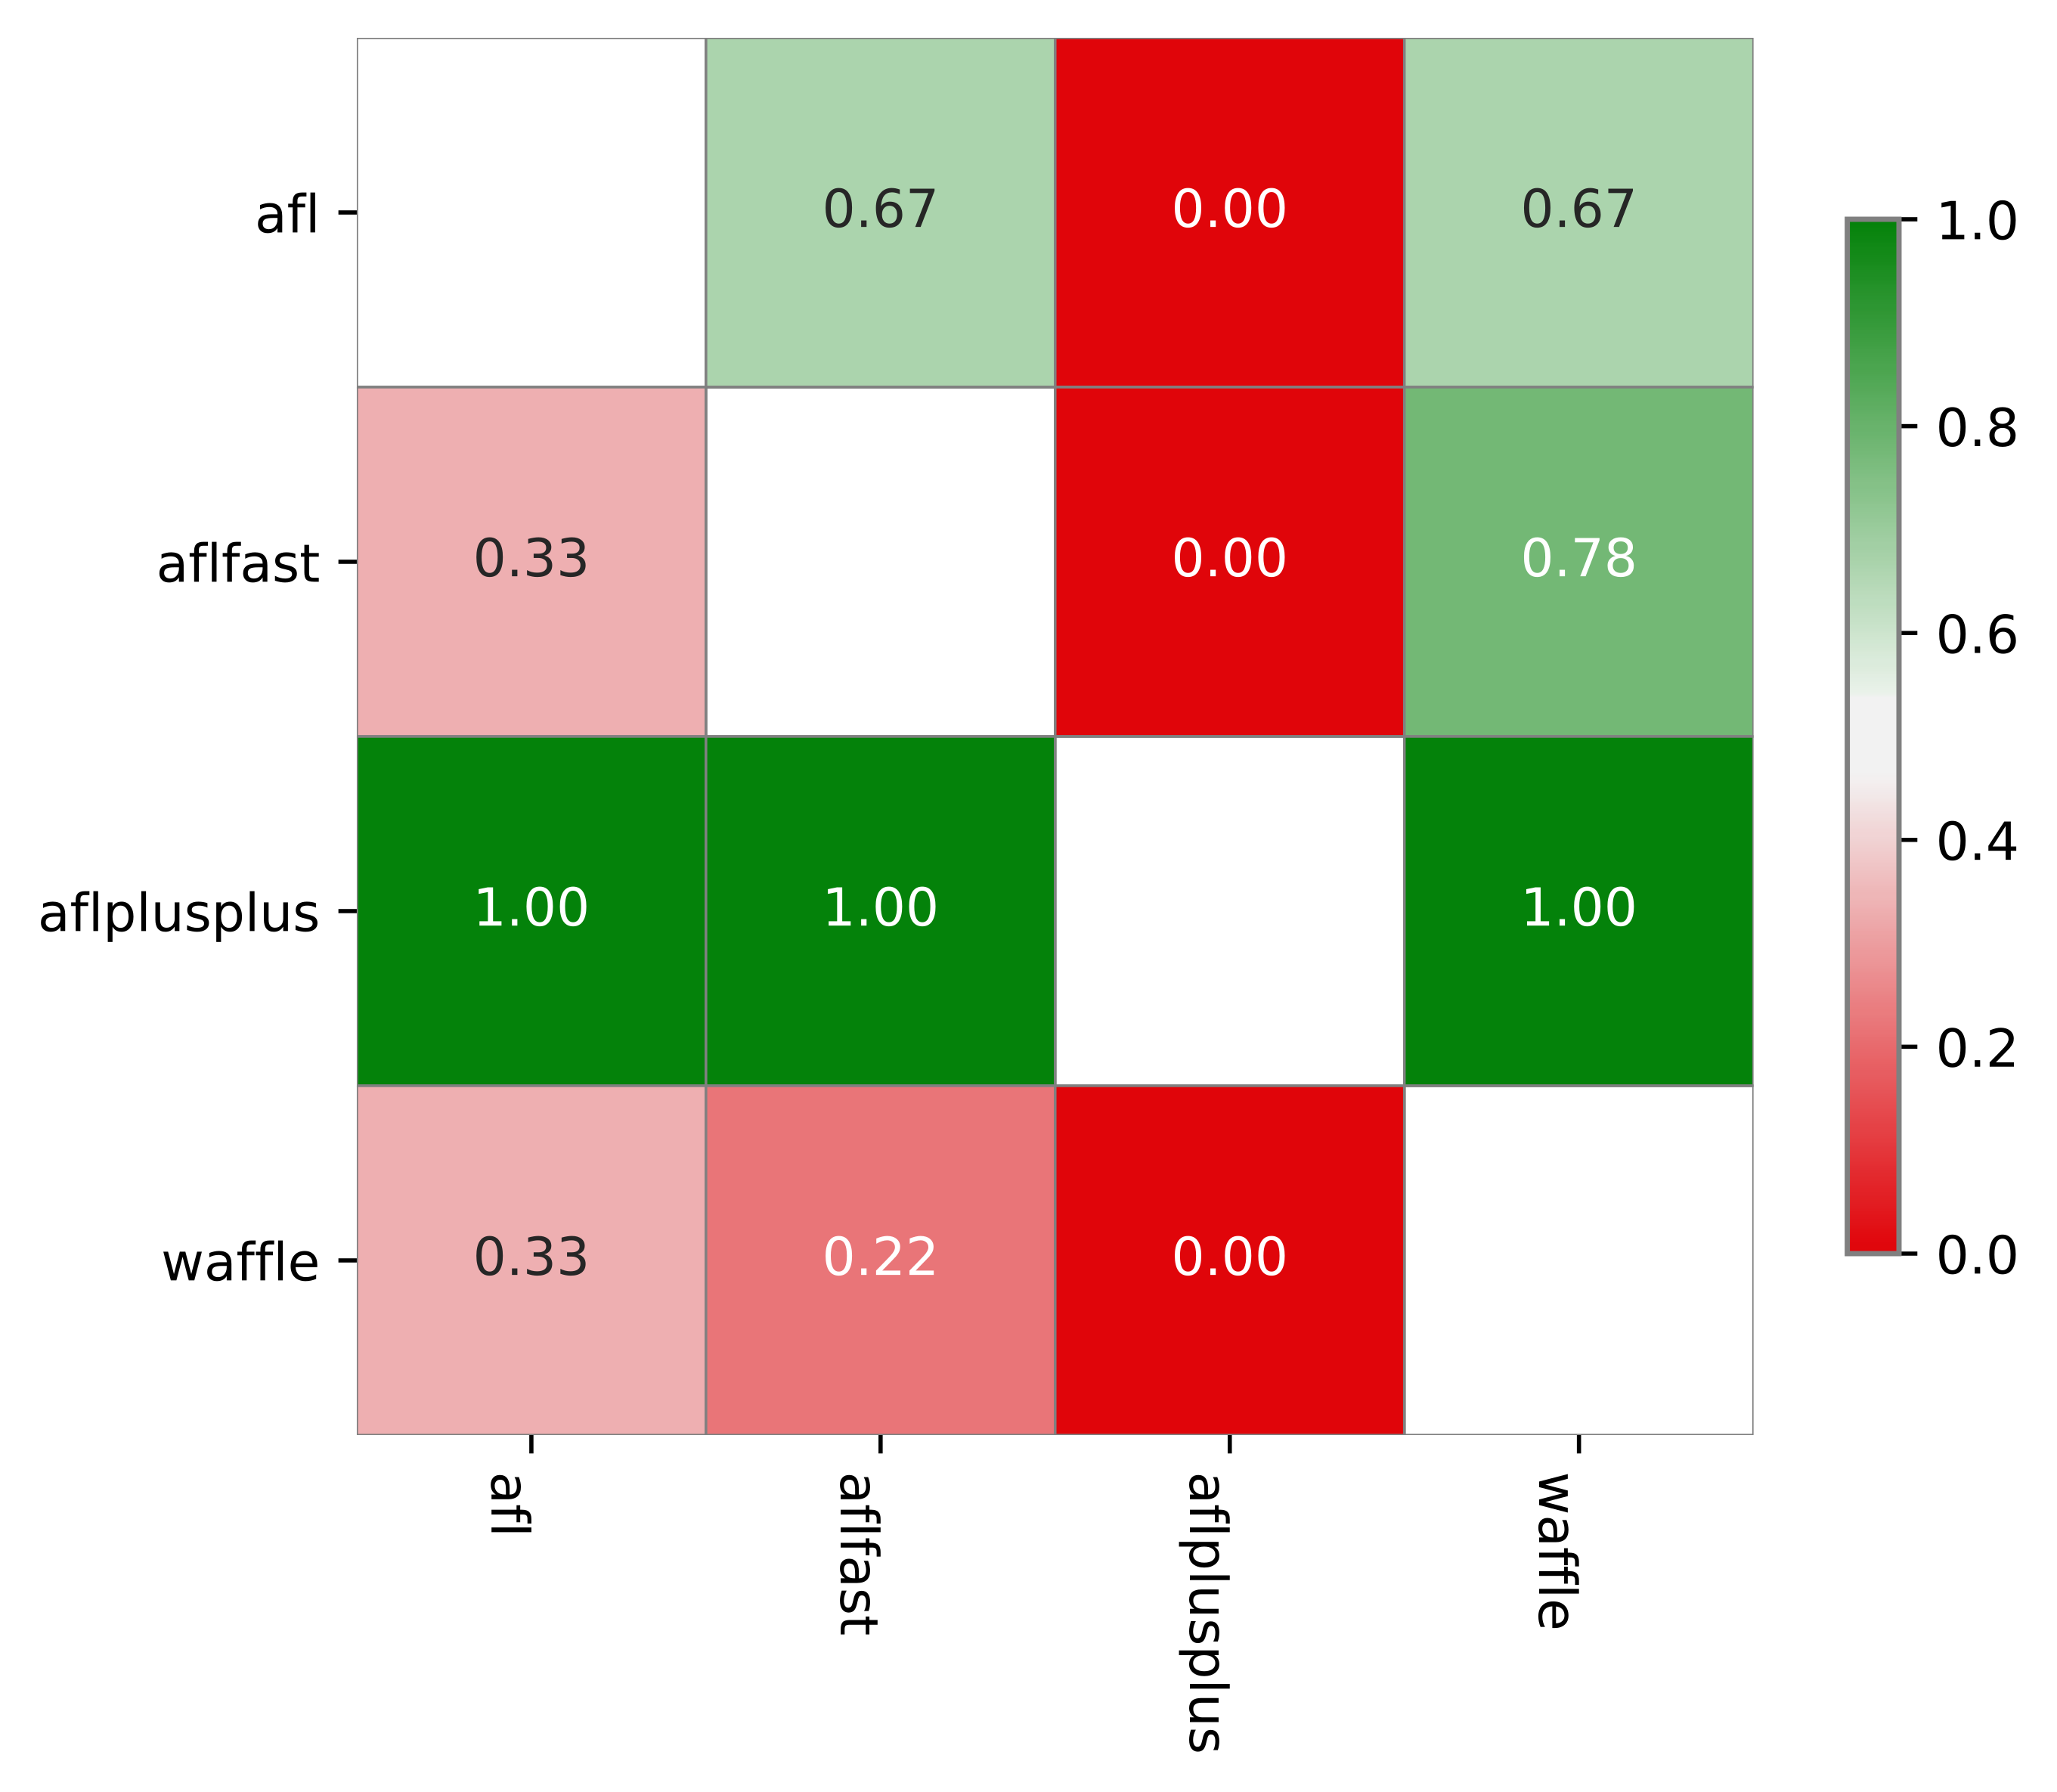
\includegraphics[width=0.95\linewidth]{Experiments/libpng-1.2.56_varga_delaney_a12_plot.png}
%         \caption{libpng-1.2.56}
%         \label{fig:sub:libpng-vda12}
%     \end{subfigure}
%     \begin{subfigure}[b]{0.475\linewidth}
%         \centering
%         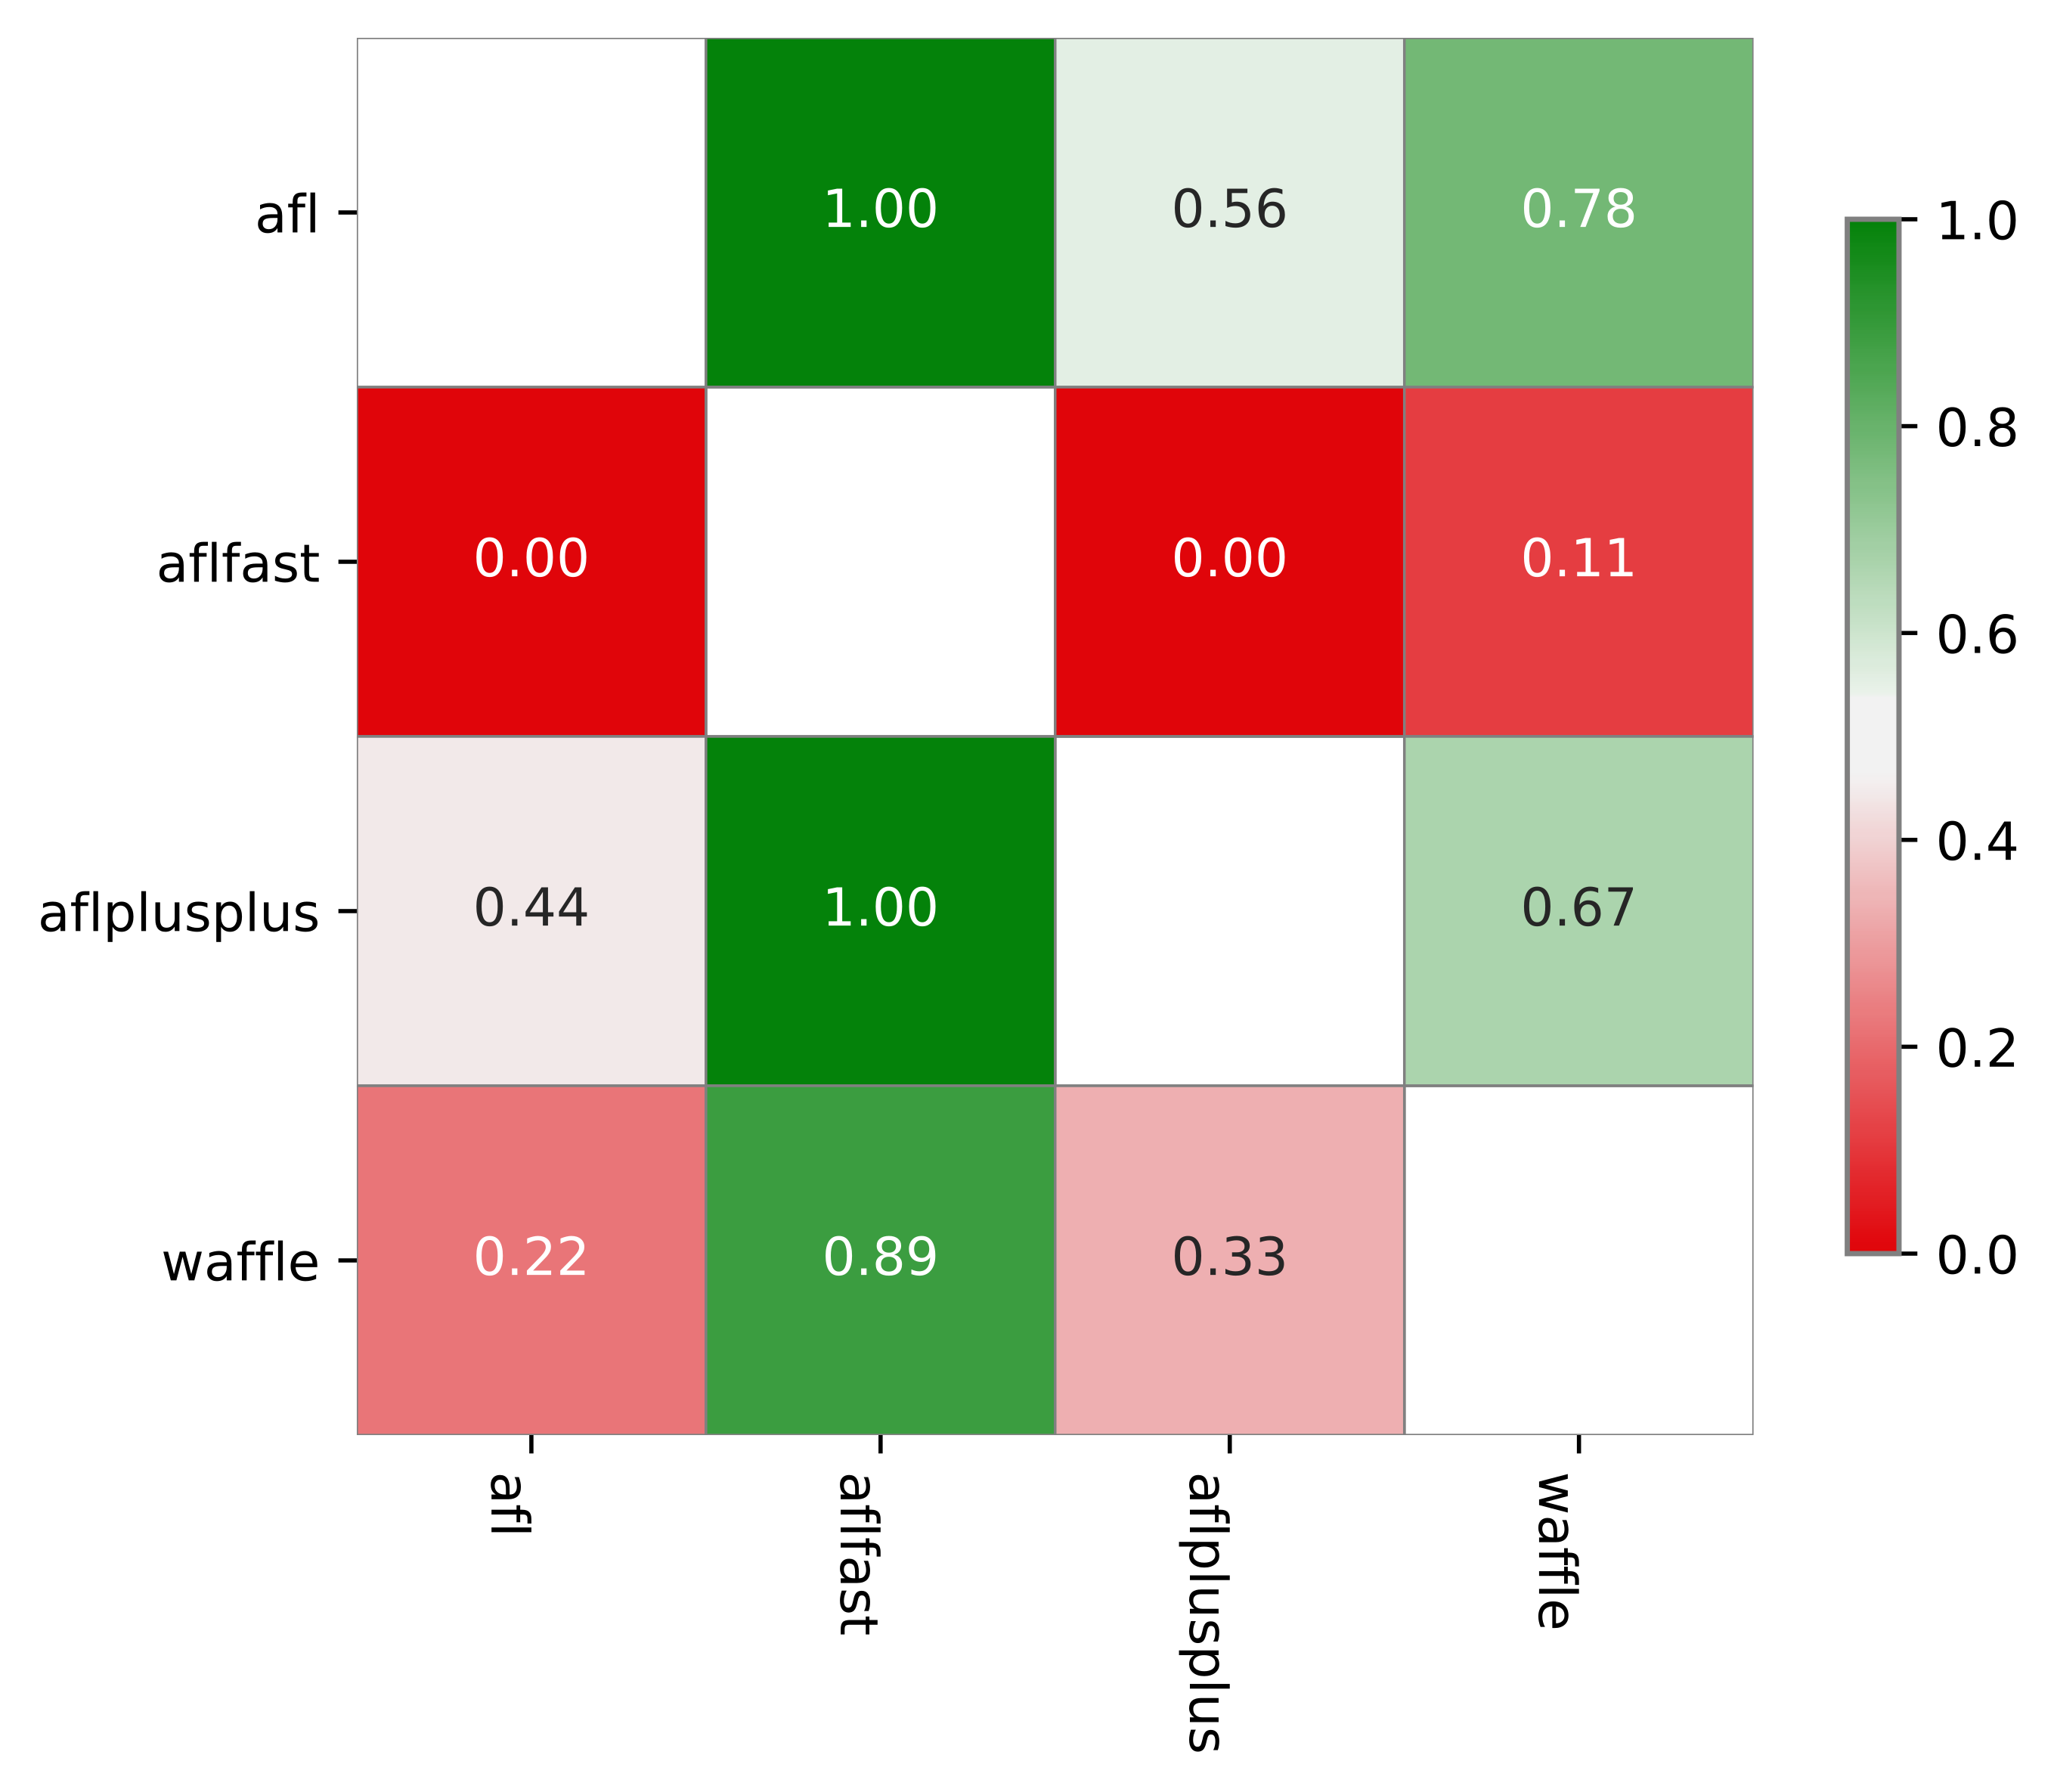
\includegraphics[width=0.95\linewidth]{Experiments/libxml2-v2.9.2_varga_delaney_a12_plot.png}
%         \caption{libxml2-v2.9.2}
%         \label{fig:sub:libxml-vda12}
%     \end{subfigure}

%     \caption{Unique coverage findings - The table summarizes the A12 values from the pairwise Vargha-Delaney A measure of effect size. Green cells indicate the probability the fuzzer in the row will outperform the fuzzer in the column.}
%     \label{fig:vda12}
% \end{figure}

% \begin{table}[!t]
%     \begin{tabular}{|l|c|c|c|c|} 
%         \hline
%         \textbf{Fuzzer}         & \textbf{Benchmarks} & \begin{tabular}[c]{@{}c@{}}\textbf{Coverage}\\ \textbf{STD}\end{tabular} & \begin{tabular}[c]{@{}c@{}}\textbf{Mean}\\ \textbf{Coverage}\end{tabular} & \begin{tabular}[c]{@{}c@{}}\textbf{Max}\\ \textbf{Coverage}\end{tabular} \\
%         \hline
%         \rowcolor{gray!20}      & freetype2 & 673.115 & 18968.3 & 19745.0 \\ \cline{2-5}
%                                 & libjpeg   & 155.094 &  3454.6 &  3628.0 \\ \cline{2-5}
%                                 \rowcolor{gray!20} & libpng    &  	0.577 &  1941.6 &  1942.0 \\ \cline{2-5}
%                                 & libxml    & 225.646 & 11246.3 & 11504.0 \\ \cline{2-5}
%         \hline
%         \rowcolor{gray!20} \multirow{4}{*}{AFL}    & freetype2 & 146.550 & 18520.0 & 18612.0 \\ \cline{2-5}
%                                 & libjpeg   &  51.156 &  3352.0 &  3411.0 \\ \cline{2-5}
%                                 & libpng    &   2.645 &  1943.0 &  1945.0 \\ \cline{2-5}
%                                 & libxml    & 355.017 & 11456.3 & 11851.0 \\ \cline{2-5}
%         \hline
%         \rowcolor{gray!20} \multirow{4}{*}{AFLFast}& freetype2 &  59.732 & 17508.0 & 17576.0 \\ \cline{2-5}
%                                 & libjpeg   &  41.761 &  3354.0 &  3402.0 \\ \cline{2-5}
%                                 & libpng    &   0.577 &  1942.3 &  1943.0 \\ \cline{2-5}
%                                 & libxml    & 152.346 & 10953.6 & 11093.0 \\ \cline{2-5}
%         \hline
%         \rowcolor{gray!20} \multirow{4}{*}{AFL++}  & freetype2 & 694.859 & 20961.3 & 21625.0 \\ \cline{2-5}
%                                 & libjpeg   & 195.438 &  3634.6 &  3749.0 \\ \cline{2-5}
%                                 & libpng    &  16.258 &  2092.6 &  2111.0 \\ \cline{2-5}
%                                 & libxml    & 84.571  & 11334.3 & 11431.0 \\ \cline{2-5}
%         \hline
%     \end{tabular}
%     \caption{Coverage stats}
%     \label{table:all-cov}
% \end{table}

Table \ref{table:all-cov} contains the coverage stats of the experiments. These stats describe an average coverage performance (on three trials) for each fuzzer on benchmarks. 

\begin{table}[!t]
    \centering
    \begin{tabular}{|c|c|c|c|c|} 
        \hline
        \textbf{Fuzzer}         & \textbf{Benchmarks} & \begin{tabular}[c]{@{}c@{}}\textbf{Coverage}\\ \textbf{STD}\end{tabular} & \begin{tabular}[c]{@{}c@{}}\textbf{Mean}\\ \textbf{Coverage}\end{tabular} & \begin{tabular}[c]{@{}c@{}}\textbf{Max}\\ \textbf{Coverage}\end{tabular} \\
        \hline
        \multirow{4}{*}{freetype}     
        & Waffle & 673.115 & 18968.3 & 19745.0 \\ \cline{2-5}
        & AFL & 146.550 & 18520.0 & 18612.0 \\ \cline{2-5}
        & AFLFast &  59.732 & 17508.0 & 17576.0 \\ \cline{2-5}
        & AFL++ & 694.859 & 20961.3 & 21625.0 \\ \cline{2-5}
        
        \hline
        \multirow{4}{*}{libjpeg}    
        & Waffle   & 155.094 &  3454.6 &  3628.0 \\ \cline{2-5}
        & AFL   &  51.156 &  3352.0 &  3411.0 \\ \cline{2-5}
        & AFLFast   &  41.761 &  3354.0 &  3402.0 \\ \cline{2-5}
        & AFL++   & 195.438 &  3634.6 &  3749.0 \\ \cline{2-5}
        
        \hline
        \multirow{4}{*}{libpng}
        & Waffle    &  	0.577 &  1941.6 &  1942.0 \\ \cline{2-5}
        & AFL    &   2.645 &  1943.0 &  1945.0 \\ \cline{2-5}
        & AFLFast    &   0.577 &  1942.3 &  1943.0 \\ \cline{2-5}
        & AFL++    &  16.258 &  2092.6 &  2111.0 \\ \cline{2-5}
        
        \hline
        \multirow{4}{*}{libxml}  
        & Waffle    & 225.646 & 11246.3 & 11504.0 \\ \cline{2-5}
        & AFL    & 355.017 & 11456.3 & 11851.0 \\ \cline{2-5}
        & AFLFast    & 152.346 & 10953.6 & 11093.0 \\ \cline{2-5}
        & AFL++    & 84.571  & 11334.3 & 11431.0 \\ \cline{2-5}
        \hline
    \end{tabular}
    \caption{Coverage stats}
    \label{table:all-cov}
\end{table}

\subsection{Execution time}

The performance of the fuzzers, based on execution times, is shown in histograms of instances of the tests (\cref{Figure:exe-freetype,Figure:exe-libjpeg,Figure:exe-libpng,Figure:exe-libxml}). In \cref{Figure:exe-freetype,Figure:exe-libpng,Figure:exe-libxml}, although the total number of findings in Waffle is less than AFL's, the Waffle's findings are spread more toward higher execution times.

\begin{figure}
    \centering
    \begin{subfigure}[t]{0.475\textwidth}
        \centering
        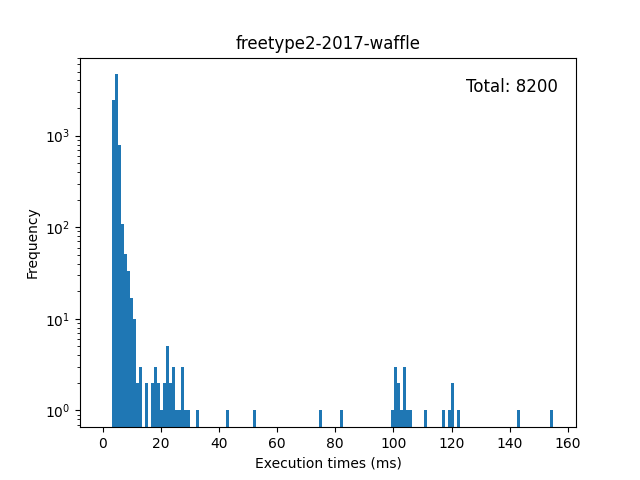
\includegraphics[width=\textwidth]{Experiments/execs/freetype2-2017-waffle.png}
        \caption{}
        \label{fig:sub:freetype-hist-waffle}
    \end{subfigure}
    \hfill
    \begin{subfigure}[t]{0.475\textwidth}
        \centering
        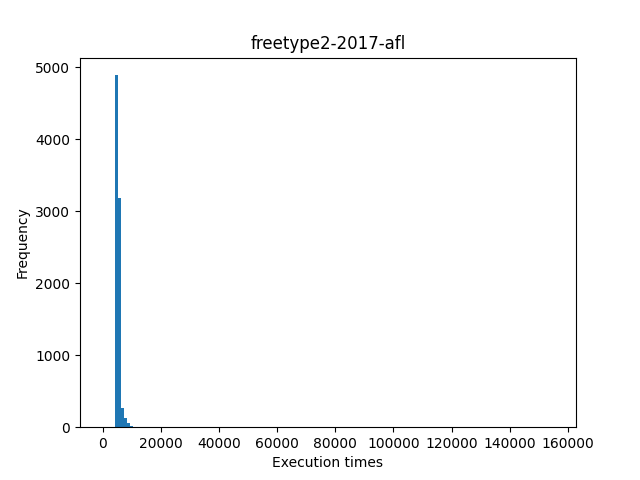
\includegraphics[width=\textwidth]{Experiments/execs/freetype2-2017-afl.png}
        \caption{}
        \label{fig:sub:freetype-hist-afl}
    \end{subfigure}
    \vskip\baselineskip
    \begin{subfigure}[t]{0.475\textwidth}
        \centering
        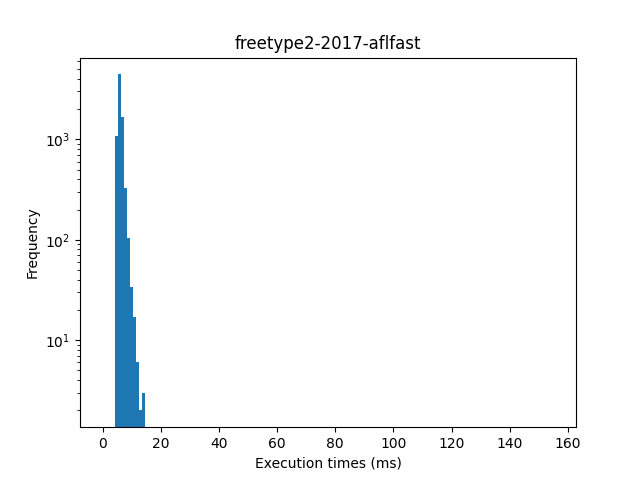
\includegraphics[width=\textwidth]{Experiments/execs/freetype2-2017-aflfast.png}
        \caption{}
        \label{fig:sub:freetype-hist-aflfast}
    \end{subfigure}
    \hfill
    \begin{subfigure}[t]{0.475\textwidth}
        \centering
        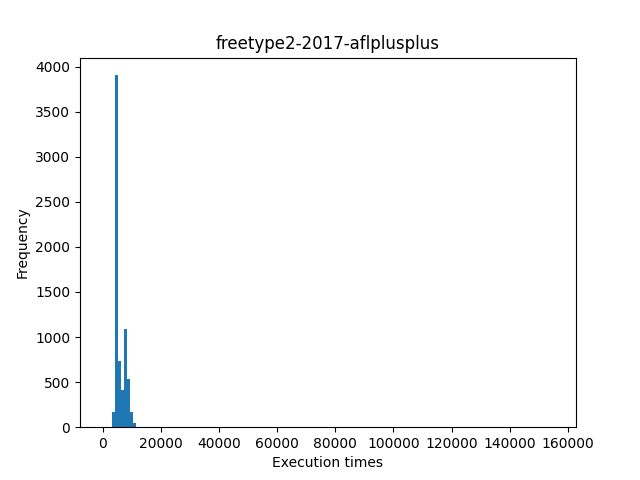
\includegraphics[width=\textwidth]{Experiments/execs/freetype2-2017-aflplusplus.png}
        \caption{}
        \label{fig:sub:freetype-hist-aflplusplus}
    \end{subfigure}

    \caption{Histogram of execution times: freetype2-2017}
    \label{Figure:exe-freetype}
\end{figure}


\begin{figure}
    \centering
    \begin{subfigure}[t]{0.475\textwidth}
        \centering
        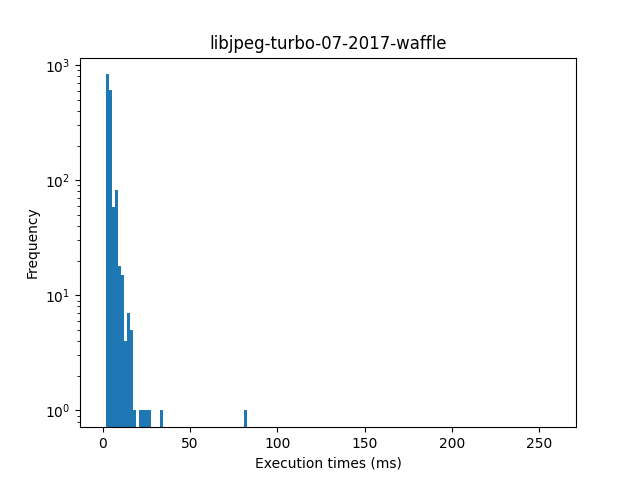
\includegraphics[width=\textwidth]{Experiments/execs/libjpeg-turbo-07-2017-waffle.png}
        \caption{}
        \label{fig:sub:libjpeg-hist-waffle}
    \end{subfigure}
    \hfill
    \begin{subfigure}[t]{0.475\textwidth}
        \centering
        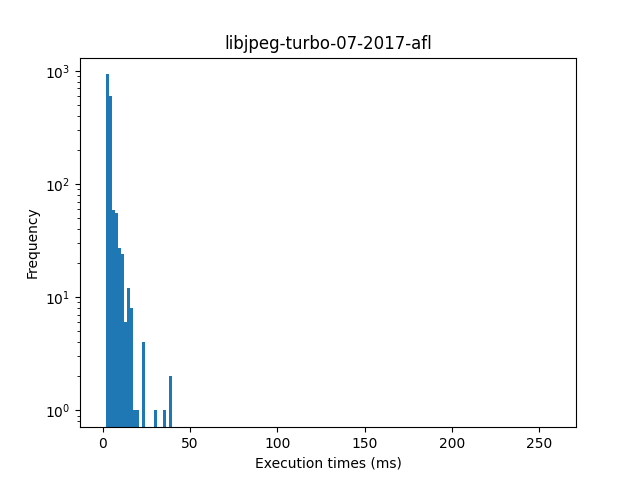
\includegraphics[width=\textwidth]{Experiments/execs/libjpeg-turbo-07-2017-afl.png}
        \caption{}
        \label{fig:sub:libjpeg-hist-afl}
    \end{subfigure}
    \vskip\baselineskip
    \begin{subfigure}[t]{0.475\textwidth}
        \centering
        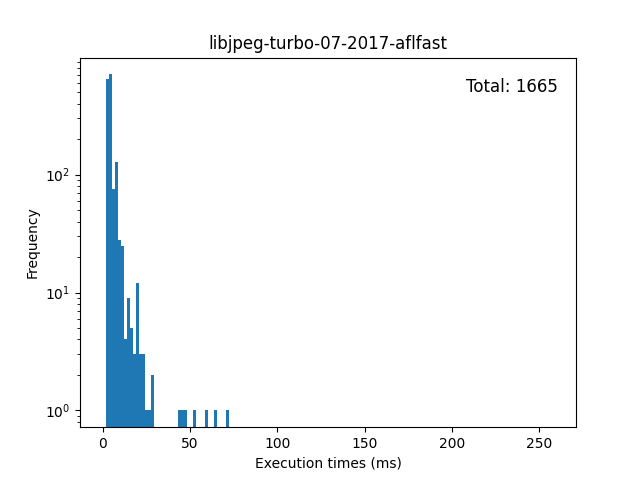
\includegraphics[width=\textwidth]{Experiments/execs/libjpeg-turbo-07-2017-aflfast.png}
        \caption{}
        \label{fig:sub:libjpeg-hist-aflfast}
    \end{subfigure}
    \hfill
    \begin{subfigure}[t]{0.475\textwidth}
        \centering
        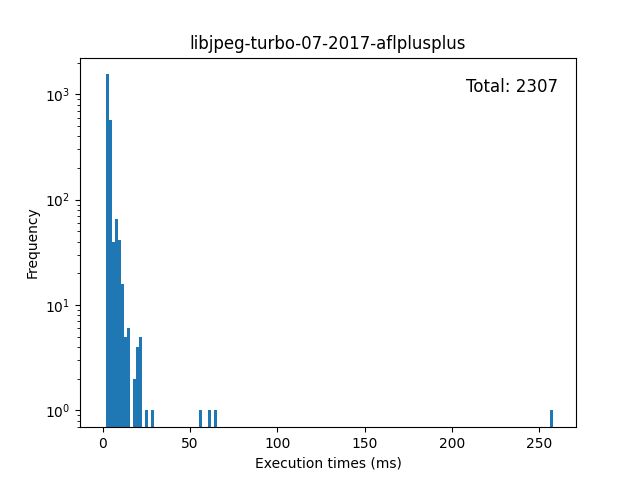
\includegraphics[width=\textwidth]{Experiments/execs/libjpeg-turbo-07-2017-aflplusplus.png}
        \caption{}
        \label{fig:sub:libjpeg-hist-aflplusplus}
    \end{subfigure}

    \caption{Histogram of execution times: libjpeg-turbo-07-2017}
    \label{Figure:exe-libjpeg}
\end{figure}

\begin{figure}
    \centering
    \begin{subfigure}[t]{0.475\textwidth}
        \centering
        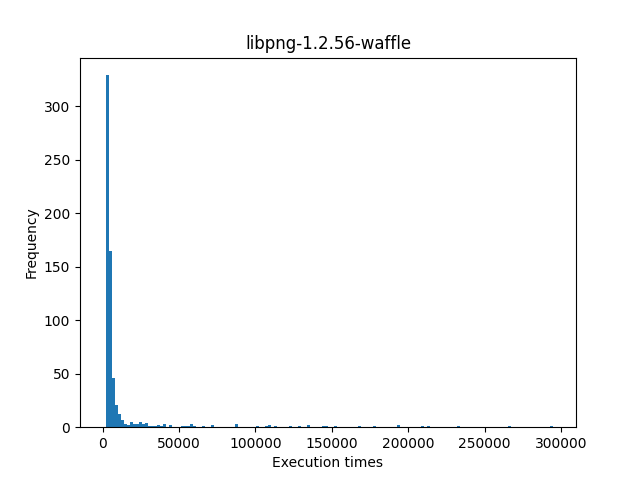
\includegraphics[width=\textwidth]{Experiments/execs/libpng-1.2.56-waffle.png}
        \caption{}
        \label{fig:sub:libpng-hist-waffle}
    \end{subfigure}
    \hfill
    \begin{subfigure}[t]{0.475\textwidth}
        \centering
        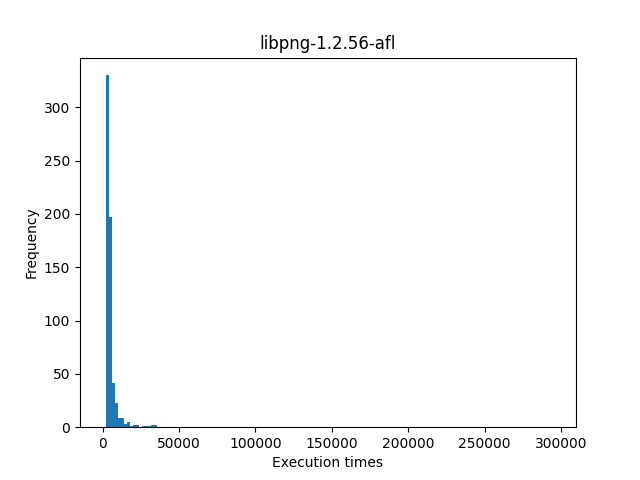
\includegraphics[width=\textwidth]{Experiments/execs/libpng-1.2.56-afl.png}
        \caption{}
        \label{fig:sub:libpng-hist-afl}
    \end{subfigure}
    \vskip\baselineskip
    \begin{subfigure}[t]{0.475\textwidth}
        \centering
        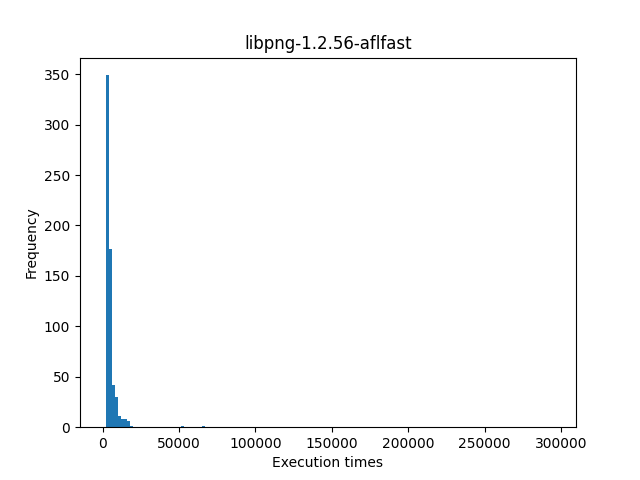
\includegraphics[width=\textwidth]{Experiments/execs/libpng-1.2.56-aflfast.png}
        \caption{}
        \label{fig:sub:libpng-hist-aflfast}
    \end{subfigure}
    \hfill
    \begin{subfigure}[t]{0.475\textwidth}
        \centering
        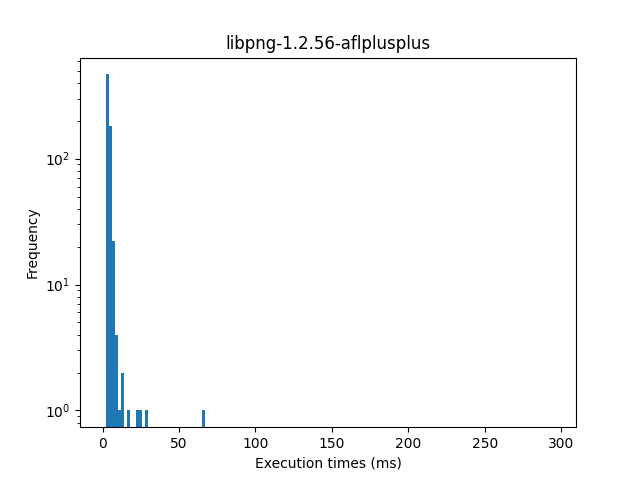
\includegraphics[width=\textwidth]{Experiments/execs/libpng-1.2.56-aflplusplus.png}
        \caption{}
        \label{fig:sub:libpng-hist-aflplusplus}
    \end{subfigure}

    \caption{Histogram of execution times: libpng-1.2.56}
    \label{Figure:exe-libpng}
\end{figure}

\begin{figure}
    \centering
    \begin{subfigure}[t]{0.475\textwidth}
        \centering
        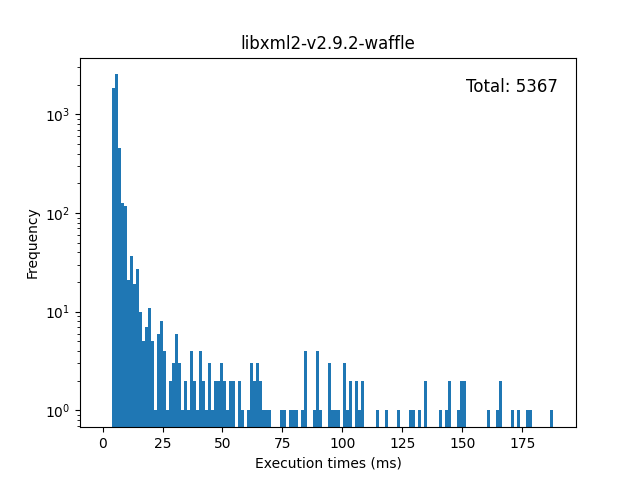
\includegraphics[width=\textwidth]{Experiments/execs/libxml2-v2.9.2-waffle.png}
        \caption{}
        \label{fig:sub:libxml2-hist-waffle}
    \end{subfigure}
    \hfill
    \begin{subfigure}[t]{0.475\textwidth}
        \centering
        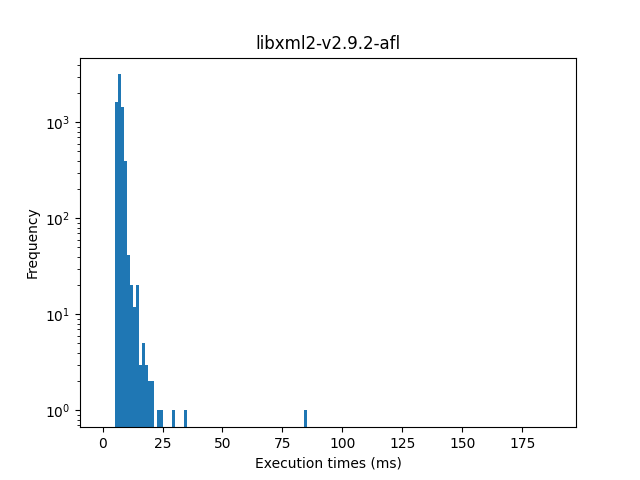
\includegraphics[width=\textwidth]{Experiments/execs/libxml2-v2.9.2-afl.png}
        \caption{}
        \label{fig:sub:libxml2-hist-afl}
    \end{subfigure}
    \vskip\baselineskip
    \begin{subfigure}[t]{0.475\textwidth}
        \centering
        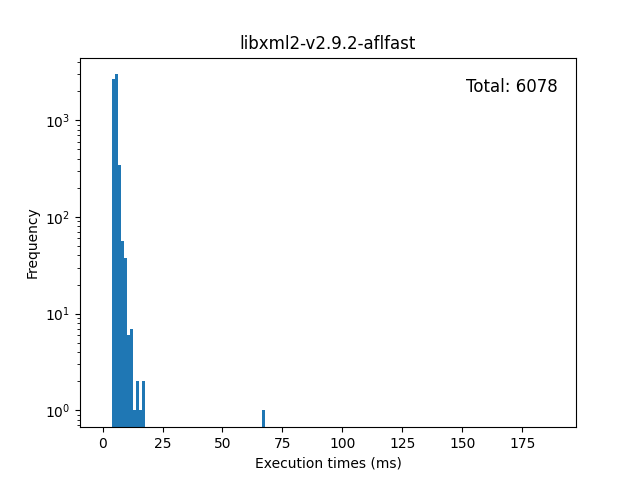
\includegraphics[width=\textwidth]{Experiments/execs/libxml2-v2.9.2-aflfast.png}
        \caption{}
        \label{fig:sub:libxml2-hist-aflfast}
    \end{subfigure}
    \hfill
    \begin{subfigure}[t]{0.475\textwidth}
        \centering
        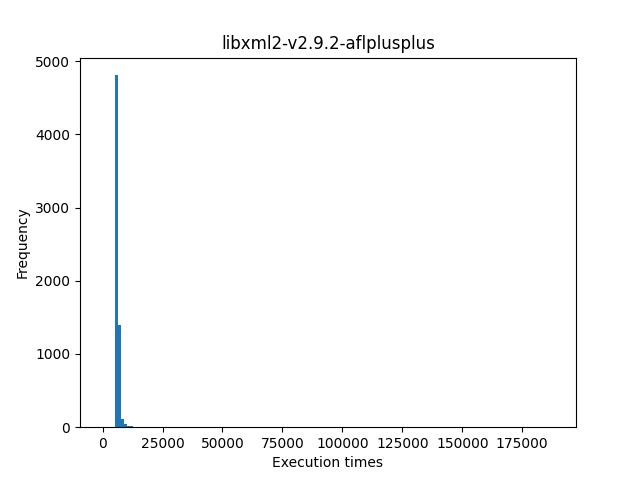
\includegraphics[width=\textwidth]{Experiments/execs/libxml2-v2.9.2-aflplusplus.png}
        \caption{}
        \label{fig:sub:libxml2-hist-aflplusplus}
    \end{subfigure}

    \caption{Histogram of execution times: libxml2-v2.9.2}
    \label{Figure:exe-libxml}
\end{figure}

Table \ref{table:all-exe} has the performance of \textbf{one} trial of each test, based on the execution time. 

\begin{table}[!t]
    \begin{adjustbox}{angle=90}
        {\setlength{\extrarowheight}{1ex}%
        \begin{tabular}{|c|c|c|c|c|c|c|c|} 
            \hline
            $Benchmarks$   & $Fuzzer$ & $Min_{(ms)}$ & $Max_{(ms)}$ & $Mean_{(ms)}$ & $Median_{(ms)}$ & $STD$ & $Total$ \\
            \hline
            \rowcolor{gray!20} \multirow{4}{*}{freetype} 
            & Waffle & 4.2 & 155.0 & 5.7 & 5.2 & 5.647 & 8201\\ \cline{2-8}
            & AFL & 4.3 & 12.7 & 5.2 & 5.0 & 0.668 & 8544 \\ \cline{2-8}
            & AFLFast & 5.4 & 14.3 & 6.7 & 6.5 & 0.831 & 7647 \\ \cline{2-8}
            & AFL++ & 3.9 & 23.1 & 5.7 & 4.9 & 1.682 & 7056 \\ \cline{2-8}
            \hline
            \rowcolor{gray!20} \multirow{4}{*}{libjpeg}
            & Waffle   & 3.1 & 81.3 & 4.6 & 3.9 & 2.884 & 1637 \\ \cline{2-8}
            & AFL   & 3.3 & 38.2 & 4.7 & 3.9 & 2.674 & 1729 \\ \cline{2-8}
            & AFLFast   & 3.3 & 71.6 & 5.3 & 4.1 & 4.374 & 1665 \\ \cline{2-8}
            & AFL++   & 3.0 & 258.8 & 4.4 & 3.7 & 6.025 & 2307 \\ \cline{2-8}
            \hline
            \rowcolor{gray!20} \multirow{4}{*}{libpng}
            & Waffle    & 2.8 & 295.1 & 12.1 & 3.9 & 31.245 & 643 \\ \cline{2-8}
            & AFL    & 2.7 & 34.8 & 5.0 & 3.8 & 3.882 & 629 \\ \cline{2-8}
            & AFLFast    & 2.9 & 64.9 & 4.9 & 3.8 & 3.967 & 635 \\ \cline{2-8}
            & AFL++    & 2.8 & 65.1 & 4.1 & 3.5 & 3.003 & 684 \\ \cline{2-8}
            \hline
            \rowcolor{gray!20} \multirow{4}{*}{libxml} 
            & Waffle    & 5.2 & 188.0 & 8.3 & 6.2 & 13.071 & 5369 \\ \cline{2-8}
            & AFL    & 6.0 & 85.0 & 7.7 & 7.5 & 1.551 & 6757 \\ \cline{2-8}
            & AFLFast    & 5.2 & 67.5 & 6.2 & 6.0 & 1.064 & 6078 \\ \cline{2-8}
            & AFL++    & 5.0 & 100.8 & 6.1 & 5.9 & 1.781 & 6426 \\ \cline{2-8}
            \hline
        \end{tabular}
        }
    \end{adjustbox}
    \caption{Execution times stats}
    \label{table:all-exe}
\end{table}
